\documentclass[12pt,oneside]{memoir} 

\usepackage[latinica, biblatex]{matfmaster} 
\usepackage{listings}
\usepackage{listings-golang}
\usepackage{color}
\usepackage{tikz}
\usepackage{pgfplots}
\usetikzlibrary{pgfplots.groupplots}
\usepackage{diagbox}
\usepackage{array}
\usepackage{fancyvrb}
\usepackage{float}
\definecolor{background}{RGB}{255, 248, 220}


\lstset{ 
    frame=single,
    basicstyle=\footnotesize,
    keywordstyle=\color{blue},
    showstringspaces=false, 
    stringstyle=\color{red},
    tabsize=4,
    language=Golang,
    literate = {==}{{~={}=~}}3
}
\renewcommand\lstlistingname{Primer}
\renewcommand\lstlistlistingname{Primer}

\lstnewenvironment{snippet}[1][]
    {\lstset{float=tpb,#1}} 
    {}



\bib{literatura}


\autor{Miloš Mitrović}
\naslov{Konkurentnost u programskom jeziku Go}
\godina{2018}
\mentor{dr Milena \textsc{Vujošević Janičić}\\ Univerzitet u Beogradu, Matematički fakultet}
\komisijaA{dr Vesna \textsc{Marinković}\\  Univerzitet u Beogradu, Matematički fakultet}
\komisijaB{dr Milan \textsc{Banković}\\  Univerzitet u Beogradu, Matematički fakultet}


\apstr{
Situacija u računarstvu u današnje vreme višejezgarnih procesora, mrežnih sistema i velikih serverskih projekata koji se mogu sastojati od nekoliko desetina miliona linija koda, značajno se razlikuje od sredine u kojoj su kreirani jezici kao što su C, C++ i Python. Programski jezik Go je upravo dizajniran sa ciljem postizanja maksimalne produktivnosti u ovakvoj sredini, na takav način da programeru maksimalno olakša sam proces razvoja softvera.

Go je statički tipizirani programski jezik koji se kompilira, sa jednostavnom sintaksom koja omogućava razvoj kvalitetnog softvera sa malim brojem linija koda. Jedna od glavnih osobina koje Go čini posebnim je njegova konkurentnost koja je ugrađena u sam jezik i na intuitivan način obezbeđuje programeru pisanje memorijski i vremenski efikasnih programa sa veoma čitljivim kodom.

Rad opisuje karakteristike jezika Go, posebno razmatra njegovu konkurentnost i daje rezultate uporednih testova konkurentnog izvršavanja implementacija izabranih algoritima u jezicima Go, C/C++ i Python. Go predstavlja jezik opšte namene, ali zbog svoje dobro realizovane konkurentnosti, pogodan je za razvoj serverskih aplikacija, pa je iz tog razloga kao primer upotrebe razvijena serverska aplikacija koja demonstrira način na koji se konkurentnost može iskoristiti, kao i pojedine druge aspekte programskog jezika.
}


\kljucnereci{programski jezik Go, konkurentno programiranje, serverska aplikacija}

\begin{document}

\frontmatter
\naslovna
\komisija
\posveta{Mojoj sestri Ivoni}
\apstrakt
\tableofcontents*
\mainmatter

\chapter{Uvod}

Programski jezik Go je projekat koji razvija kompanija Google od 2007. godine. Postao je javno dostupan kao projekat otvorenog koda 2009. godine i u stalnom je razvoju. Cilj projekta je bio kreirati novi statički tipiziran jezik koji se kompilira, a koji bi omogućavao jednostavno programiranje kao kod interpretiranih, dinamički tipizarnih programskih jezika. 

Smatra se da Go pripada C familiji programskih jezika, ali pozajmljuje i adaptira ideje raznih drugih jezika, izbegavajući karakteristike koje dovode do komplikovanog i nepouzdanog koda. Iako nije objektno-orijentisan, Go podržava određene koncepte kao što su metodi i interfejsi koji pružaju fleksibilnu apstrakciju podataka. Go omogućava efikasnu konkurentnost koja je ugrađena u sam jezik, kao i automatsko upravljanje memorijom, odnosno sakupljanje smeća. 

Zbog svojih osobina kao što je konkurentnost, Go je posebno dobar za izradu različitih vrsta serverskih aplikacija, ali je pre svega jezik opšte namene pa se može koristiti za rešavanje svih vrsta problema. Ima primenu u raznim oblastima kao što su grafika, mobilne aplikacije, mašinsko učenje i još mnoge druge. Osim kompanije Google, koristi se u velikom broju drugih kompanija kao alternativa jezicima poput Python-a i Javascript-a, jer pruža znatno viši stepen efikasnosti i bezbednosti.

U radu su istražene i opisane karakteristike programskog jezika Go (glava \ref{g2}), sa akcentom na njegove mogućnosti za konkurentno programiranje (glava \ref{conc}). Implementirana su konkurentna rešenja izabranih algoritama u programskim jezicima Go, C/C++, Python, i urađena je uporedna analiza vremenskih i memorijskih zahteva u  zavisnosti od dimenzije problema i broja jezgara na kojima se softver izvršava (glava \ref{g4}). Kao primer upotrebe, razvijena je serverska aplikacija koja demonstrira korišćenje konkurentnosti kao i drugih aspekata jezika Go (glava \ref{app}).

% GO OPIS==============================================================================

\chapter{Karakteristike programskog jezika Go} \label{g2}

U ovoj glavi opisane su karakteristike i osnovni koncepti programiranja jezika Go.  Konkurentnost jezika je detaljnije opisana i njoj je posvećena glava \ref{conc}.

\section{Go alat}

Alat \texttt{go} predstavalja osnovni alat za upravljanje Go kodovima. Neke od definisanih komandi u okviru alata su: \texttt{build} za kompilaciju paketa, \texttt{run} za kompilaciju i izvršavanje Go programa, \texttt{test} za testiranje paketa, \texttt{get} za preuzimanje i instaliranje paketa, \texttt{fmt} za formatiranje koda paketa. Alat se upotrebljava \texttt{go komanda [argumenti]} notacijom.

\section{Početni primer}

Početni program \textit{Hello World} u jeziku Go prikazan je u primeru \ref{lst:hello}. Na početku programa navodi se naziv paketa. Svaki paket koji sadrži \texttt{main} funkciju mora nositi naziv \texttt{main}. Sa naredbom \texttt{import} navode se nazivi svih paketa koji se koriste u programu. Go ne dozvoljava uključivanje suvišnih paketa, već se mogu navesti samo paketi koji se upotrebljavaju u programu. Ukoliko se navede paket koji se ne koristi, biće prijavljena greška tokom kompilacije. Nakon svake naredbe nije obavezno navođenje znaka \texttt{;} , osim ako je potrebno navesti više naredbi u istoj liniji. Komentari se navode na isti način kao u jeziku C.

\begin{center}
\begin{lstlisting}[caption=Program \textit{Hello World} u jeziku Go,label={lst:hello},  backgroundcolor=\color{background}]
package main

import "fmt"

func main() {
	fmt.Println("Hello World!") // ispisuje Hello World!
}
\end{lstlisting}
\end{center}

\section{Tipovi podataka}

Go je statički tipiziran jezik što znači da se promenljivoj dodeljuje tip prilikom njene deklaracije i on se ne može menjati tokom izvršavanja programa. Za razliku od C-a, Go ne podržava automatsku konverziju tipova vrednosti već se konverzija vrednosti mora navesti eksplicitno, u suprotnom prijavljuje se greška prilikom kompilacije. Pravilo koje važi za pakete važi i za promenljive, svaka deklarisana promenljiva mora biti upotrebljena.

Program prikazan u primeru \ref{lst:add} prikazuje definiciju i deklaraciju različitih vrsta promenljivih. Tip promenljive se ne mora eksplicitno navesti, već se može zaključiti na osnovu dodele operatorom \texttt{:=} kada se promenljiva uvodi. Iako nije definisana, promenljiva \texttt{a} ima podrazumevanu vrednost koja je za numeričke tipove 0.

\begin{center}
\begin{lstlisting}[caption=Program koji ilustruje rad sa promenljivama, label={lst:add},  backgroundcolor=\color{background}]
package main

import "fmt"

func main() {
	var a float32
	b := 5
	var c int

	c = int(a) + b
	fmt.Println(c)	 // 5
}
\end{lstlisting}
\end{center}

\newpage

Tipovi podataka koji su definisani u programskom jeziku Go mogu se klasifikovati u četiri kategorije \cite{bookGoProg}: 
\begin{enumerate}
\item Osnovni tipovi  (numerički, bulovski, tekstualni)
\item Složeni tipovi (nizovi i strukture)
\item Referentni tipovi (pokazivači, isečci, mape, kanali, funkcije)
\item Interfejsni tipovi (interfejsi)
\end{enumerate}

Konstante (\texttt{const}) u Go-u predstavljaju izraze čija je vrednost unapred poznata kompilatoru i čija se evaluacija izvršava tokom kompilacije, a ne tokom izvršavanja programa. Konstante se mogu definisati samo za osnovne tipove podataka. 

\subsection{Osnovni tipovi podataka}

Osnovni tipovi koji postoje u programskom jeziku Go, podeljeni su na:
\begin{itemize}

\item Numeričke -  celobrojne označene (\texttt{int8}, \texttt{int16}, \texttt{int32}, \texttt{int64}),
 celobrojne neoznačene  (\texttt{uint8}, \texttt{uint16}, \texttt{uint32}, \texttt{uint64}), u pokretnom zarezu (\texttt{float32}, \texttt{float64}) i kompleksne (\texttt{complex64}, \texttt{complex128})

\item Bulovske  (\texttt{bool})

\item Tekstualne (\texttt{string})

\end{itemize}


Paket \texttt{strings} pruža veliki broj funkcija za manipulaciju tipom \texttt{string}. Iako u okviru paketa postoji funkcija \texttt{Compare(string, string)}, Go dozvoljava poređenje stringova operatorom \texttt{==}, kao i ostalim relacionim operatorima.
\\

Operatori koji su definisani u Go-u podeljeni su u sledeće kategorije:
\begin{itemize}

\item Aritmetički operatori ( \texttt{+} ,  \texttt{-} , \texttt{*} ,  \texttt{/} ,  \texttt{\%} ,  \texttt{++} ,   \texttt{-{}-} )
\item Relacioni operatori ( \texttt{==} ,  \texttt{!=} ,  \texttt{>} ,  \texttt{<} ,  \texttt{>=} ,  \texttt{<=})
\item Logički operatori (\texttt{\&\& },  \texttt{||} ,  \texttt{!})
\item Bitski operatori ( \texttt{\&} ,  \texttt{|} ,  \texttt{\^} ,  \texttt{>{}>} ,  \texttt{<{}<})
\item Operatori dodele ( \texttt{=} ,  \texttt{+=} ,  \texttt{-=} ,  \texttt{*=} ,  \texttt{/=} ,  \texttt{\%=} ,   \texttt{>{}>=} ,  \texttt{<{}<=} ,  \texttt{\&=} ,  \texttt{|=} ,  \texttt{\^{}=} )

\end{itemize}

Upotreba nad određenim tipovima podataka, uloga i arnost Go operatora, definisani su na isti način kao u jeziku C.

\subsection{Složeni tipovi podataka}
U složene tipove podatka u programskom jeziku Go spadaju \textbf{nizovi} i \textbf{strukture}.
\\

\textbf{Niz} predstavlja sekvencu elemenata istog tipa, fiksne dužine. Elementima niza se pristupa standardnom \texttt{[indeks]} notacijom gde prvi element ima indeks 0. Ugrađena funkcija \texttt{len(niz)} koristi se za dobijanje podatka o dužini niza. Dužina niza se mora navesti prilikom deklaracije ili, ukoliko se izvršava i inicijalizacija, umesto dužine može se navesti znak \texttt{...} , a dužina će biti zaključena na osnovu incijalizacije.

Go dozvoljava poređenje nizova iste dužine definisanih nad istim tipom podataka, relacionim operatorima \texttt{==} i \texttt{!=} . Dva niza su jednaka ako imaju jednake vrednosti na istim pozicijama. Primer \ref{lst:arr_str} prikazuje definisanje i upotrebu niza.
\\

\textbf{Strukture} su složeni podaci koji grupišu nula ili više elemenata ne obavezno istih tipova. Svaki element mora biti jedinstveno imenovan i predstavlja jedno polje strukture. Definisanjem strukture definiše se novi tip podataka korišćenjem ključne reči \texttt{type} ispred same definicije strukture. Poljima strukture pristupa se pomoću znaka \texttt{.} i naziva polja. Prazne strukture \texttt{struct\{\}} mogu se koristiti za komunikaciju preko kanala u slučajevima kada nije bitan sadržaj poruke već samo davanje signala. U implementaciji serverske aplikacije u glavi \ref{app} u potpoglavlju \ref{appFile} prikazan je primer upotrebe praznih struktura za realizaciju semafora. 

Ugnježdavanje struktura je dozvoljeno, odnosno definisanje struktura koje sadrže druge strukture kao polja. Strukture istog tipa mogu se porediti relacionim operatorima   \texttt{==} i \texttt{!=} . Dve strukture su jednake ako imaju jednake vrednosti na istim poljima. Nad strukturama se mogu definisati metodi koji su opisani u poglavlju \ref{metod}. Primer \ref{lst:arr_str} demonstrira rad sa strukturama.

Prilikom alociranja memorije za nizove i strukture umesto deklarisanja promenljivih, može se koristiti ugrađena funkcija \texttt{new} koja vraća pokazivač na alocirani niz ili strukturu. Nizovi se funkcijama prosleđuju kao kopija, ne preko reference kao što je slučaj u drugim jezicima poput C-a. Prenošenje niza preko reference, mora se eksplicitno naglasiti korišćenjem pokazivača. U tom slučaju, pristupanje vrednostima niza unutar funkcije postiže se korišćenjem operatora \texttt{*} odnosno notacijom \texttt{(*naziv)[indeks]}. Ukoliko se funkciji prosledi struktura preko reference, poljima se može pristupiti uobičajenom notacijom upotrebom znaka \texttt{.} i naziva polja.
\newpage

\begin{center}
\begin{lstlisting}[caption=Rad sa nizovima i strukturama, label={lst:arr_str},  backgroundcolor=\color{background}]
	var a [3]int
	b := [...]int{1, 2, 3}
	a[0] = 1
	fmt.Println(a == b) // false

	type Point struct{ X, Y int }
	p1 := Point{1, 2}
	p2 := Point{Y:2}
	p2.X = 1
	fmt.Println(p1 == p2) // true

	c := new([3]int)
	c[0] = 1
	fmt.Println(a == *c) // true			
\end{lstlisting}
\end{center}

\subsection{Referentni tipovi podataka}
U referentne tipove podataka spadaju \textbf{pokazivači}, \textbf{isečci}, \textbf{mape}, \textbf{kanali} i \textbf{funkcije}. U ovom segementu, opisani su svi referentni tipovi podataka osim funkcija, kojima je posvećeno potpoglavlje \ref{func}, i kanala, koji su opisani u glavi \ref{conc} čija je tema konkurentnost, u poglavlju \ref{chanel}. 
\\

\textbf{Pokazivač} referiše na vrednost neke promenljive koja se trenutno čuva u memoriji. Pokazivači kao vrednost čuvaju lokaciju promenljive u memoriji na koju referišu. Za dobijanje lokacije promenljive, koristi se operator \texttt{\&}. Za dereferenciranje pokazivača, odnosno dobijanje vrednosti na koju pokazivač referiše, koristi se operator \texttt{*}.
\\

\textbf{Isečak} (engl. "slice") u programskom jeziku Go, predstavlja pogled na elemente niza. Za razliku od nizova, isečci su promenljive dužine. Svaki isečak se sastoji od tri podatka: pokazivača na niz, dužine i kapaciteta. Sintaksa za rad sa isečcima je ista kao i za rad sa nizovima, osim što prilikom deklaracije nije potrebno navoditi dužinu isečka. Za alociranje isečaka koristiti se ugrađena funkcija \texttt{make([]tip, dužina, kapacitet)}. Funkcija kreira isečak koji sadrži onoliko elemenata kolika mu je zadata dužina, koji su postavljeni na podrazumevane vrednosti. Kapacitet isečka nije fiksan, a za podatak o njegovoj trenutnoj vrednosti koristi se ugrađena funkcija \texttt{cap(isečak)}.

\begin{figure}
\begin{center}
\includegraphics[scale=0.33]{slice.png}
\end{center}
\caption{Poziv funkcije \texttt{append} kada postoji i kada ne postoji dovoljno prostora za dodavanje}
\label{fig:slice}
\end{figure}

\begin{center}
\begin{lstlisting}[caption=Rad sa isečcima, label={lst:slice},  backgroundcolor=\color{background}]
	a := [...]int{1, 2, 3, 4, 5}
	
	s1 := a[:3] 				
	fmt.Println(s1, cap(s1))	// [1 2 3] 5
	
	s1 = append(s1, 6) 			// [1 2 3 6]
	a[0] = 10					// deluje i na s1
	s2 := make([]int, 4, 4)		// [0 0 0 0] 
	copy(s2, s1)
	s1[1] = 11					// ne deluje na s2
	
	fmt.Println(s1, cap(s1)) 	// [10 11 3 6] 5
	fmt.Println(s2, cap(s2)) 	// [10 2 3 6] 4
	
	s1 = append(s1, 7, 8)		// realocira s1
	a[2] = 12					// ne deluje na s1
	fmt.Println(s1, cap(s1))	// [10 11 3 6 7 8] 12
\end{lstlisting}
\end{center}

Definisanje isečka nad nizom postiže se korišćenjem \texttt{niz[od:do]} notacije, pri čemu se gornja granica ne uključuje. Ukoliko se donja granica izostavi, donja granica je početak niza, ukoliko se gornja granica izostavi, gornja granica je kraj niza, a ukoliko se navede samo znak \texttt{:} , isečak će sadržati sve elemente niza. 

Za rad sa isečcima postoji ugrađena funkcija \texttt{copy(destinacija, izvor)} koja kopira elemente jednog isečka u drugi i kao rezultat vraća broj kopiranih elemenata. Maksimalan broj elemenata koji će biti kopiran, jednak je dužini kraćeg isečka. Dozvoljeno je da isečci pre kopiranja dele elemente. Funkcija \texttt{append(isečak, elementi)} koristi se za dodavanje elemenata isečku. Tokom rada ukoliko ne postoji dovoljno mesta, funkcija može imati potrebu da realocira niz i zbog toga kao rezultat vraća ažuriranu referencu na isečak. Nakon poziva funkcije \texttt{append} moguće je da isečci koji su delili elemente niza, pokazuju na različite nizove, što je i prikazano na slici \ref{fig:slice} \cite{bookGoProg}. Primer \ref{lst:slice} ilustruje rad sa isečcima.
\\

\textbf{Mapa} je referentni tip podataka koji referiše na heš tabelu. U tabeli se čuvaju parovi ključ - vrednost, pri čemu je vrednost svakog ključa jedinstvena. Svi ključevi su istog tipa i sve vrednosti su istog tipa. Jedini uslov je da se tip ključa može porediti operatorom \texttt{==} , dok vrednosti mogu biti proizvoljnog tipa, uključujući i druge mape. 

Funkcija \texttt{make(map[tip\_ključa] tip\_vrednosti)} se koristi prilikom alociranja prostora za novu mapu. Upis u mapu postiže se \texttt{naziv[ključ] = vrednost} notacijom. Ugrađena funkcija \texttt{delete(mapa, ključ)} koristi se za brisanje parova iz mape. Funkcija kao parametre ima naziv mape i ključ para koji se briše. Ukoliko ključ ne postoji, funkcija nema nikakav efekat. Dodeljivanje vrednosti promenljivoj na osnovu ključa iz mape postiže se \texttt{v := naziv[ključ]} notacijom, pri čemu ukoliko ključ ne postoji, vrednost \texttt{v} će biti postavljena na podrazumevanu. Moguće je izvršiti proveru da li je određeni ključ definisan u mapi upotrebom \texttt{v, ok := naziv[ključ]} ili  \texttt{\_, ok := naziv[ključ]} notacije, gde je \texttt{ok} promenljiva tipa \texttt{bool} koja nosi informaciju da li ključ postoji ili ne. 

\begin{center}
\begin{lstlisting}[caption=Rad sa mapama, label={lst:map},  backgroundcolor=\color{background}]
	m1 := make(map[string]int)
	m1["a"] = 1
	m2 := map[string]float32{"m": 1.23, "a": 2.34}
	
	_, ok := m2["b"]
	delete(m2, "p")		// nema efekta
	delete(m2, "a")
	fmt.Println(m2, ok) // [m:1.23] false
\end{lstlisting}
\end{center}

U programskom jeziku Go, operacije nad mapama nisu atomične i prilikom konkurentnog korišćenja potrebno je koristiti odgovarajuće mere sigurnosti koje su opisane u glavi \ref{conc}. Primer \ref{lst:map} demonstrira rad sa mapama.



\section{Naredbe za kontrolu toka}

U programskom jeziku Go, naredbe za kontrolu toka izvršavanja su \texttt{if}, \texttt{switch}, \texttt{for} i \texttt{defer}. Sintaksa naredbe \texttt{if} prikazana je u primeru \ref{lst:if}. U naredbi \texttt{if} pre uslova moguće je navesti jednu naredbu koja je razdvojena znakom \texttt{;} od uslova kao kod \texttt{for} petlje. 

\begin{center}
\begin{lstlisting}[caption=Sintaksa naredbe \texttt{if}, label={lst:if},  backgroundcolor=\color{background}]
	if inicijalizacija; uslov1 {
		// naredbe
	} else if uslov2 {
		// naredbe
	} else {
		// naredbe
	}
\end{lstlisting}
\end{center}

Naredba \texttt{switch} omogućava ispitivanje vrednosti izraza po slučajevima i njena sintaksa je prikazana u primeru \ref{lst:switch}. Ukoliko je vrednost izraza jednaka nekom od slučajeva, izvršiće se deo koda naveden nakon znaka \texttt{:} , do definicije sledećeg slučaja ili kraja naredbe. U suprotnom izvršava se slučaj \texttt{default}, ako je naveden. Ukoliko se na kraju slučaja navede \texttt{fallthrough} naredba, izvršava se i k\^{o}d slučaja direktno ispod. Za pojedinačni slučaj moguće je navoditi više vrednosti razdvojenih zarezima. 

\begin{center}
\begin{lstlisting}[caption=Sintaksa naredbe \texttt{switch}, label={lst:switch},  backgroundcolor=\color{background}]
	switch izraz {
    case vrednost1:
        // naredbe
    case vrednost2, vrednost3:
       	// naredbe
    default:
      	// naredbe
    }
\end{lstlisting}
\end{center}


Jedina petlja koja postoji u programskom jeziku Go jeste \texttt{for} i njena sintaksa je prikazana u primeru \ref{lst:for}. Za izlazak iz petlje koristi se naredba \texttt{break}, a za prelazak na sledeću iteraciju naredba \texttt{continue}. Petlja \texttt{for} se može koristiti zajedno sa naredbom \texttt{range} za iteriranje kroz sekvencijalne strukture kao što su nizovi, isečci i mape. 

\begin{center}
\begin{lstlisting}[caption=Sintaksa \texttt{for} petlje, label={lst:for},  backgroundcolor=\color{background}]
	for inicijalizacija; uslov; inkrementacija; { 
		// naredbe
	}

	for indeks, vrednost := range sekvencijalna_struktura {
		// naredbe
	}
\end{lstlisting}
\end{center}


Naredba \texttt{defer} odlaže izvršavanje navedene funkcije do trenutka završetka funkcije u kojoj se nalazi. Argumenti funkcije se određuju u trenutku navođenja naredbe \texttt{defer}, samo je izvršavanje funkcije odloženo. Naredba garantuje da će se funkcija izvršiti i u slučaju dolaska do greške. 

\begin{center}
\begin{lstlisting}[caption=Primer koji demonstrira upotrebu kontrolnih struktura, label={lst:control},  backgroundcolor=\color{background}]
	a := [...]uint{1, 2, 3}
	if len(a) > 1 {
		for i,v := range a {	
			fmt.Println(i,v) // indeks, vrednost
		}
	}

	switch a[2] {
    case 3:
        fmt.Println("bigger than two")
		fallthrough
    case 2:
        fmt.Println("bigger than one")
    default:
        fmt.Println("one")
    }
\end{lstlisting}
\end{center}

Najčešća upotreba naredbe \texttt{defer} je za operacije koje se obavljaju u paru, kao što je otvaranje i zatvaranje datoteka. Odmah nakon otvaranja datoteke moguće je naredbom \texttt{defer} pozvati funkciju za zatvaranje datoteke, čime se garantuje da će se datoteka zatvoriti i doprinosi čitljivijem kodu. 

Naredbe \texttt{if} i \texttt{for} zahtevaju upotrebu vitičastih zagrada i u slučajevima kada se u bloku nalazi samo jedna naredba, a uslove nije potrebno navoditi unutar zagrada. Primer  \ref{lst:control} ilustruje upotrebu standardnih kontrolnih struktura. 

Osim navedenih kontrolnih struktura Go podržava i \texttt{go to} naredbe u kombinaciji sa labelama. Generalno, upotreba \texttt{go to} naredbi nije preporučena jer dovodi do loše strukture i nečitljivog koda.


\section{Funkcije} \label{func}

Funkcije u programskom jeziku Go predstavljaju referentni tip podataka. Sintaksa za definisanje funkcije prikazana je u primeru \ref{lst:funcDef}. Lista parametara se navodi u formatu \texttt{naziv tip}, a ukoliko postoji više parametara istog tipa za redom dovoljno je navesti njihov tip samo jedanput. Ukoliko je lista rezultata jednočlana, nije potrebno navoditi zagrade.

\begin{center}
\begin{lstlisting}[caption=Sintaksa za definisanje funkcije, label={lst:funcDef},  backgroundcolor=\color{background}]
func naziv(lista parametara) (lista rezultata) {
	telo funkcije 
} 
\end{lstlisting}
\end{center}

Osim što mogu imati proizvoljan broj argumenata, funkcije mogu imati više povratnih vrednosti. Postoje i \textit{varijadičke funkcije}, odnosno funkcije sa promenljivim brojem argumenata. Varijadičke funkcije definišu se upotrebom znaka \texttt{...} ispred tipa argumenta koji se može pojaviti nula ili više puta. 

Omogućeno je definisanje funkcija unutar funkcija gde unutrašnja funkcija ima pristup svim promenljivama spoljašnje funkcije, kao i  definisanje \textit{anonimnih funkcija}, odnosno funkcija bez imena koje se izvršavaju na mestu gde su definisane. Funkcije predstavljaju tipove prvog reda i mogu se prosleđivati drugim funkcijama i dodeljivati promenljivama. Primer \ref{lst:func} demonstrira rad sa funkcijama.

\begin{center}
\begin{lstlisting}[caption=Rad sa funkcijama, label={lst:func},  backgroundcolor=\color{background}]
func add(args ...int) int {
	sum := 0
	for _, v := range args {
		sum += v
	}
	return sum
}
func calc(x, y int) (int, int) {
	add := func() int { return x + y }
	sub := func() int { return x - y }

	return add(), sub()
}	
func power(x int) func(int)int {
	res := 1
	return func(a int)int {
		for i:=0; i<a; i++ {
			res *= x
		}
		return res
	}
}

func main() {
	fmt.Println(add(1,2,3))		// 6
	fmt.Println(calc(1,2)) 		// 3, -1
	fmt.Println(power(2)(4))	//16
}
\end{lstlisting}
\end{center}

\section{Metodi}  \label{metod}

U programskom jeziku Go ne postoji pojam klase, ali je omogućeno definisanje metoda nad korisnički definisanim tipovima. Metod predstavlja običnu funkciju koja u sebi sadrži specijalni \textit{prijemnik} (engl. "receiver") za tip podataka nad kojim je metod definisan. Metod se definiše na isti način kao i funkcija, osim što se prijemnik navodi između ključne reči \texttt{func} i naziva metoda.

Pozivanje metoda postiže se navođenjem znaka \texttt{.} i naziva metoda nakon promenljive za koju je potrebno pozvati metod. Ukoliko metod menja podatke promenljive nad kojom je pozvan, potrebno je koristiti prijemnik sa referencom, odnosno navesti znak \texttt{*} ispred tipa prijemnika. 
 
Go nema definisane nivoe vidljivosti  pomoću ključnih reči kao što su \texttt{public}, \texttt{private} i \texttt{protected}. Jedini mehanizam za kontrolu vidljivosti je sledeći: svi identifikatori koji počinju velikom slovom, biće eksportovani van paketa, svi identifikatori koji počinju malim slovom, neće biti eksportovani van paketa \cite{bookGoProg}. Isto pravilo važi i za polja strukture. Na taj način struktrure nad kojima su definisani metodi mogu da oponašaju klase i enkapsulaciju podataka. Primer \ref{lst:metod} demonstrira rad sa metodima.

\begin{center}
\begin{lstlisting}[caption=Rad sa metodima, label={lst:metod},  backgroundcolor=\color{background}]
type Point struct{ X, Y float64 }

func (p Point) Distance(q Point) float64 {
	return math.Sqrt((p.X-q.X)*(p.X-q.X)+(p.Y-q.Y)*(p.Y-q.Y))
}

func (p *Point) Translate(x, y float64) {
	p.X += x
	p.Y += y
}

func main() {
	p1 := Point{0,0}
	p2 := Point{1,1}

	fmt.Println(p1.Distance(p2)) // 1.41421...
	p2.Translate(5,2)
	fmt.Println(p2)				// {6 3}
}
\end{lstlisting}
\end{center}

\section{Interfejsi}

Interfejsi se koriste kao dodatno sredstvo apstrakcije i enkapsulacije podataka. Tip interfejs definisan je kao skup potpisa metoda. Svaki interfejs se sastoji od vrednosti i konkretnog tipa. Vrednost tipa interfejs može biti bilo koja vrednost čiji tip implentira zadate metode. Konkretni tipovi su svi tipovi podataka osim interfejsa.

Tip zadovoljava neki interfejs ukoliko implementira sve metode koje taj interfejs zahteva. Unutar interfejsa moguće je navoditi i nazive drugih interfejsa koji takođe moraju biti zadovoljeni. Svi tipovi zadovoljavaju prazan interfejs (\texttt{interface\{\}}). Mnogi paketi i funkcije koriste interfejse kao što je već viđeni paket \texttt{fmt} sa interfejsom \texttt{Stringer} koji se koristi za definisanje ispisa određenog tipa podataka. Greške, koje su opisane poglavlju \ref{error}, takođe predstavljaju interfejs. Primer \ref{lst:inter} demonstrira rad sa interfejsima.

\begin{center}
\begin{lstlisting}[caption=Rad sa interfejsima, label={lst:inter},  backgroundcolor=\color{background}]
type geometry interface { 
	area() float64 
}
type rect struct {width, height float64}
type circle struct {radius float64}

func (r rect) area() float64 {
	return r.width * r.height
}
func (c circle) area() float64 {
	return math.Pi * c.radius * c.radius
}
func measure(g geometry) {
	fmt.Println(g, g.area())
}

func main(){
	r := rect{width: 3, height: 4}	
	c := circle{radius: 5}			
	measure(r)	//{3 4} 12 
  	measure(c)	//{5} 78.5398 
}
\end{lstlisting}
\end{center}

Pretpostavljanje tipova (engl. "type assertion") omogućava pristup konkretnom tipu u okviru interfejsa što se postiže sa \texttt{i.(T)}, gde je \texttt{i} promenljiva tipa interfejs, a \texttt{T} naziv konkretnog tipa. Ukoliko se pretpostavi pogrešan tip dolazi do greške.  Za proveru da li interfejs sadrži određeni tip prilikom pretpostavljanja mogu se vratiti dve vrednosti, vrednost tipa i vrednost \texttt{bool} koja sadrži informaciju da li je pretpostavljanje uspešno. Za obradu pojedinačnih slučajeva za svaki od mogućih tipova može se koristiti naredba \texttt{switch}.  Primer \ref{lst:type} demonstrira pretpostavljanje tipova.

\begin{center}
\begin{lstlisting}[caption=Pretpostavljanje tipova kod interfejsa, label={lst:type},  backgroundcolor=\color{background}]
	var i interface{} = "hello"

	s := i.(string)
	fmt.Println(s) 		// hello

	s, ok := i.(string)
	fmt.Println(s, ok) 	// hello true

	f, ok := i.(float64)
	fmt.Println(f, ok) 	// 0 false
\end{lstlisting}
\end{center}


\section{Refleksija}

U računarstvu, refleksija predstavlja sposobnost programa da izvrši ispitivanje svoje strukture i ponašanja u toku izvršavanja. Refleksija se može koristiti za ispitivanje tipova promenljivih tokom izvršavanja u zavisnosti od čega program može da preduzme odgovarajuće akcije. Go podržava refleksiju tipova koja je omogućena upotrebom paketa \texttt{reflect}.

Unutar paketa, definisani su tipovi \texttt{Type} i \texttt{Value}, funkcija \texttt{TypeOf(promenljiva)} za dobijanje informacije o tipu promenljive i funkcija \texttt{ValueOf(promenljiva)} za dobijanje vrednosti promenljive. Funkcije kao argument prihvataju tip \texttt{interface\{\}}. 

Za postavljanje vrednosti postoje metodi \texttt{Set(vrednost)} za svaki tip podataka koji se poziva nad tipom \texttt{Value}, kao i metod \texttt{CanSet()} za proveru da li je moguće postaviti vrednost datoj promenljivoj. Vrednost je moguće postaviti samo referentnim tipovima, odnosno promeniti vrednost na koju oni referišu. Metodi \texttt{Set} se ne mogu pozivati nad promenljivom \texttt{Value} bez pripreme, već je nad njom prvo potrebno pozvati metod \texttt{Elem()} koji omogućava pristup vrednosti na koju promenljiva referiše.  

Primer \ref{lst:ref} demonstrira osnovnu upotrebu refleksije. Paket nudi još veliki broj drugih funkcija za refleksiju tipova i njihovu manipulaciju \cite{reflect}.

Refleksija predstavlja jak alat ukoliko se upotrebljava na pravi način, ali trebalo bi je koristiti sa oprezom. Postoji nekoliko razloga za opreznost: mogućnost dolaska do greške u toku izvršavanja programa koja bi mogla biti prijavljena tokom kompilacije ukoliko program ne bi koristio refleksiju; smanjena čitljivost koda ukoliko program previše koristi refleksiju; sporije izvršavanje funkcija koje koriste refleksiju naspram funkcija specijalizovanih za pojedinačne tipove \cite{bookGoProg}.

 \begin{center}
\begin{lstlisting}[caption=Osnovna upotreba refleksije, label={lst:ref},  backgroundcolor=\color{background}]
	var x float64 = 3.14
	v := reflect.ValueOf(&x) 
	
	fmt.Println(v.Type())	// *float64
	fmt.Println(v.CanSet())	// false
	
	v = v.Elem()
	fmt.Println(v.CanSet())	// true
	
	v.SetFloat(3.15)
	fmt.Println(x)			// 3.15
\end{lstlisting}
\end{center}

\section{Upravljanje greškama} \label{error}

Stanje greške u programskom jeziku Go označava se vrednostima \texttt{error}. Tip \texttt{error} predstavlja ugrađeni interfejs koji zahteva implementiranje metoda \texttt{Error()} koji kao rezultat vraća \texttt{string} sa informacijom o grešci. Ako neka funkcija kao rezultat vraća tip \texttt{error}, njegova vrednost će biti \texttt{nil} ukoliko nije došlo do greške. 

Implementacijom metoda \texttt{Error} za neki tip moguće je definisati novi tip greške. Ukoliko se upotrebljava već postojeći tip \texttt{error}, za definisanje poruke greške koristi se funkcija \texttt{New} iz paketa \texttt{errors}. Primer \ref{lst:error} demonstrira upravljanje greškama.

Na ovaj način omogućeno je elegantno upravljanje greškama. Za prekidanje toka izvršavanja u slučaju ozbiljnijih grešaka i nepredviđenih situacija koristi se ugrađena funkcija \texttt{panic(string)}. Ukoliko funkcija \texttt{F} pozove funkciju \texttt{panic} njeno izvršavanje se prekida, a zatim se izvršavaju \texttt{defer} pozivi funkcija nakon čega se funkcija \texttt{F} vraća svom pozivaocu. Tada se za pozivaoca funkcija \texttt{F} ponaša kao poziv funkcije \texttt{panic} i proces se ponavlja dokle god sve funkcije u tekućoj gorutini ne prestanu sa radom i dok sam program ne prekine sa izvršavanjem. Gorutine su osnovne jedinice izvršavanja u Go-u i predstavljaju niti niže kategorije. Gorutinama je posvećeno poglavlje \ref{gorut} u  glavi \ref{conc} koja se bavi konkurentnim programiranjem.  Ugrađene funkcije obično pozivaju funkciju \texttt{panic} ukoliko dođe do neke nepredviđene greške ili situacije koja se nije mogla otkriti tokom faze kompilacije, ali moguće je pozvati funkciju i manuelno. 

\begin{center}
\begin{lstlisting}[caption=Upravljanje greškama, label={lst:error},  backgroundcolor=\color{background}]
//definisanje novog tipa
type MyError struct {
	When time.Time
	What string
}
func (e MyError) Error() string {
	return fmt.Sprintf("%v: %v", e.When, e.What)
}
//funkcija koja koristi novi tip
func divide1(a,b float64) (float64, error) {
	if b == 0 {
		return 0, &MyError{time.Now(),"division by zero"}
	}else {
		return a/b, nil
	}
}
//funkcija koja koristi error tip
func divide2(a,b float64) (float64, error) {
	if b == 0 {
		return 0, errors.New("Division by zero")
	}else {
		return a/b, nil
	}
}
//provera greske u funkciji main
func main() {
	if v1, err := divide1(3.14,0); err != nil {
		fmt.Println(err)				
	}
	if v2, err := divide2(3.14,0); err != nil {
		fmt.Println(err)			
	}
}
\end{lstlisting}
\end{center}

Pored funkcije \texttt{panic} postoji i ugrađena funkcija \texttt{recover()} koji služi za preuzimanje kontrole gorutine koje je u stanju \texttt{panic}. Funkciju \texttt{recover} ima jedino smisla koristiti unutar naredbe \texttt{defer}. Ukoliko je tekuća gorutina u stanju \texttt{panic}, \texttt{recover} funkcija će preuzeti vrednost koju je dobila funkcija \texttt{panic} i nastaviti normalno izvršavanje programa.
 
\section{Sakupljanje smeća}

Programski jezik Go ima automatsko upravljanje memorijom odnosno sakupljanje smeća (engl. "garbage collection"). Sakupljač skenira memoriju, pronalazi objekte na koje više ne postoji ni jedna referenca i nakon toga ih briše i oslobađa memoriju. Upotrebom paketa \texttt{runtime},  sakupljač se može eksplicitno pozvati korišćenjem funkcije \texttt{GC()}. 

Od verzije Go 1.5,  sakupljač smeća \cite{garbage} kreiran je kao konkurentni, trobojni, označi-počisti (engl. "mark-sweep") sakupljač. Kod trobojnih sakupljača svaki objekat je bele, sive ili crne boje i hip segement se posmatra kao jedan povezani graf. Hip segment predstavlja segement memorije u kome se dinamčki alociraju podaci tokom izvršavanja programa.

Na početku ciklusa, svi objekti su beli. Sakupljač prvo posećuje sve korene grafa koji predstavljaju objekte kojima se može pristupiti direktno iz aplikacije, kao što su globalne promenljive i promenljive na steku, koje boji u sivo. Nakon toga, sakupljač bira neki od sivih objekata, boji ga u crno i proverava da li poseduje pokazivače ka drugim objektima. Ukoliko pronađe pokazivač ka belom objektu, označava ga sivom bojom. Proces se ponavlja dokle god postoje sivi objekti. Na kraju, belom bojom su označeni objekti do kojih nije moguće doći, odnosno objekti na koje niko ne referiše.

\begin{figure}
\begin{center}
\includegraphics[scale=0.33]{tricolor.png}
\end{center}
\caption{Prikaz označavanja objekata kod trobojnog algoritma}
\label{fig:tricolor}
\end{figure}

Čitav ovaj proces izvršava se konkurentno sa aplikacijom koja se još naziva i mutator jer menja pokazivače dok je sakupljač aktivan. Mutator ne sme da narušava pravilo da nijedan crni objekat ne pokazuje na beli kako sakupljač ne bi izgubio evidenciju objekata koji su ubačeni u deo hipa koji je već posetio. Za očuvanje ovog pravila zadužena je barijera za pisanje (engl. "write barrier") koja predstavlja funkciju koja se aktivira prilikom promene pokazivača na hipu. Barijera označava beli objekat kao sivi ukoliko u tom trenutku postoji neki pokazivač koji pokazuje na njega, čime se osigurava da će ga pre ili kasnije sakupljač obraditi, odnosno proveriti da li poseduje pokazivače ka drugim objektima. Šematski prikaz trobojnog algoritma prikazan je na slici \ref{fig:tricolor}.

Sakupljač obavlja što veći deo posla konkurentno, međutim potrebno je na kratko da zaustavi sve (engl. "stop the world") kako bi proverio potencijalne izvore sivih objekata. Pronalaženje pravog trenutka za zaustavljanje i njegovo samo trajanje, poboljšava se svakom novom distribucijom jezika Go. Od verzije Go 1.8, pauze uobičajeno traju manje od 100 mikrosekundi, a često se dešava da je njihovo trajanje samo 10 mikrosekundi, što je značajno unapređenje od verzije Go 1.5 gde su pauze trajale nekoliko milisekundi.

\section{Testiranje}

Go ima ugrađenu podršku za automatsko testiranje paketa. Testiranje se izvršava pomoću alata \texttt{go test} i paketa \texttt{testing}. Alat se koristi za testiranje funkcija i kao rezultat daje vrednosti \texttt{PASS} ili \texttt{FAIL}. Benčmark funkcije za testiranje performansi su takođe podržane. Sa alatom dolazi veliki broj flegova koji omogućava različite opcije kao što su broj ponavljanja benčmark testova ili broj korišćenih procesora prilikom testiranja. Testovi se izdvajaju u posebnu test datoteku. 

Funkcije za testiranje u nazivu imaju prefiks \texttt{Test}, a zatim naziv funkcije koju testiraju. Kao argument funkcije imaju parametar \texttt{T} koji se koristi za obaveštavanje o neuspešnim testovima i logovanje dodatnih informacija. Benčmark funkcije imaju prefiks \texttt{Benchmark}, a kao argument imaju parametar \texttt{B} koji poseduje veliki broj istih metoda kao i parametar \texttt{T}, sa dodatnim stavkama koje su potrebne za merenje performansi kao što je polje \texttt{N} koje označava broj ponavljanja operacije koja se testira.

Alat \texttt{go test} takođe podržava i funkcije primere (engl. "example functions") čija je primarna uloga dokumentacija koda. Funkcije primeri imaju prefiks  \texttt{Example}, a kao argument nemaju nikakve parametre i ne vraćaju nikakav rezultat. Alat prevodi i izvršava ove funkcije, a ukoliko imaju neki ispis, on se ispisuje na standardnom izlazu. Pod komentarom koji počinje sa \texttt{Output:} moguće je navesti ispis funkcije koji će biti upoređen sa ispisom funkcije na standardnom izlazu. Primer \ref{lst:test} prikazuje različite tipove funkcija za testiranje.

\begin{center}
\begin{lstlisting}[caption=Različiti tipovi funkcija za testiranje, label={lst:test},  backgroundcolor=\color{background}]
// funkcija koja se testira
func Sum(x int, y int) int {  
	return x + y
}
// funkcija za testiranje
func TestSum(t *testing.T) {  
	total := Sum(1, 2)
	if total != 3 {
		t.Errorf("Sum was incorrect, got: %d, want: %d.", total, 3)
	}
}
// benchmark funkcija
func BenchmarkSum(b *testing.B) {
	for i := 0; i < b.N; i++ {
		Sum(2,2)
	}
}
// example funkcija
func ExampleSum() {
	fmt.Println(Sum(5,0))
	fmt.Println(Sum(1,3))
	// Output:
	// 5
	// 4
}

\end{lstlisting}
\end{center}

\section{Paketi}

U okviru same distribucije programskog jezika Go postoji veliki broj paketa standardne biblioteke koji obezbeđuju različite usluge. Neki od osnovnih paketa su upotrebljeni u primerima: \texttt{fmt} za formatirani ulaz/izlaz; \texttt{strings} za rad sa stringovima; \texttt{math} sa implementacijama matematičkih funkcija. Još jedan paket koji se često upotrebljava je paket \texttt{os} koji predstavlja interfejs ka operativnom sistemu i omogućava funkcionalnosti kao što su rad sa sistemom datoteka, pristup argumentima komandne linije i pokretanje procesa.

U standardnoj biblioteci takođe postoje paketi za rad sa SQL bazama podataka, kriptografskim funkcijama, kompresiju podataka, rad sa slikama,  podršku za mrežno programiranje i još mnogi drugi. Pored paketa standardne biblioteke postoje dodatni i prošireni paketi u okviru Go projekta koji imaju labavije uslove kompatibilnosti Go verzija. Ovde se mogu pronaći paketi za razvoj aplikacija za mobilne platforme, eksperimentalni debager, prošireni kriptografski i mrežni paketi. 

Paketi van distribucije samog jezika mogu se preuzeti korišćenjem komande \texttt{go get} i navođenjem repozitorijuma u kome se paket nalazi. Na veb sajtu \url{https://godoc.org/} mogu se naći paketi i njihove dokumentacije koje razvijaju članovi Go zajednice koja vremenom postaje sve veća. Paketi su odobreni od strane Go projekta i mogu se naći paketi koji obezbeđuju najrazličitije alate za programiranje kao i API-je mnogih postojećih servisa.


% KONKURENTNO==============================================================================
\chapter{Konkurentno programiranje u jeziku Go} \label{conc}

U ovoj glavi objašnjeni su osnovni pojmovi i problemi koji se javljaju kod konkurentnog programiranja. Nakon toga, opisano je kako je konkurentnost realizovana u programskom jeziku Go, kako se ona upotrebljava i načini na koje se rešavaju određeni problemi. 

\section{Osnovni pojmovi konkurentnog programiranja}

U računarstvu, \textit{konkurentnost} označava mogućnost procesa da određene delove izvršava nezavisno jedne od drugih, bez uticanja na sam rezultat programa. Pojam konkurentnosti se često poistovećuje sa \textit{paralelizmom}. Za razliku od konkurentnosti, paralelizam podrazumeva da se delovi jednog procesa izvršavaju istovremeno, dok konkurentnost samo definiše celine koje se mogu izvršavati u preklapajućim vremenskim intervalima, ali ne obavezno istovremeno. 

\subsection{Niti}

Osnovni pojam u konkurentnom programiranju predstavlja \textit{nit}. Niti su osnovne jedinice izvršavanja u okviru procesa. Jedan proces se može sastojati od više niti koje se izvršavaju konkurentno. Niti jednog procesa dele određene resurse kao što su k\^{o}d segement, segement podataka i hip segment, ali poseduju i sopstvene resurse kao što je stek. 

Korišćenje niti donosi mnoge prednosti kao što su ušteda memorijskog prostora i vremena. Niti zauzimaju manje prostora nego pojedinačni procesi jer dele određene resurse i kao rezultat se kreiraju znatno brže od procesa. Takođe, niti omogućavaju aplikacijma da obavljaju druge, nezavisne zadatke dok su neki delovi blokirani ili zauzeti. Serverske aplikacije često koriste kreiranje niti umesto kreiranja procesa za svakog novog korisnika jer se niti brže kreiraju i zauzimaju manje prostora, pa je omogućeno da se brže odgovori na zahteve i opsluži veći broj korisnika \cite{os}.  

\subsection{Mogući problemi pri konkurentnom izvršavanju}

Osim prednosti koje konkurentnost donosi, postoje problemi koji se mogu javiti pri manipulaciji zajedničkim podacima i resursima. Nekontrolisano pristupanje zajedničkim podacima može dovesti do neispravnih rezultata. Ukoliko su neki resursi deljeni, kao na primer standardni izlaz, nesinhronizovani ispis može proizvesti ispreplitane, nečitljive poruke. Situacija u kojoj krajnji rezultat zavisi od redosleda izvršavanja koraka različitih procesa ili niti koji manipulišu zajedničkim podacima ili resursima naziva se \textit{trka za resursima} (engl. "race condition") \cite{os}.

Na slici \ref{fig:race} levo, prikazan je jednostavan primer u kome se javlja problem trke za resursima. Problem se javlja jer uvećanje vrednosti deljene promenljive ne predstavlja atomičnu operaciju. Promena vrednosti podrazumeva, čitanje tekuće vrednosti i pravljenje lokalne kopije, uvećanje vrednosti lokalne kopije i na kraju izmenu originalne vrednosti. U primeru, nit 1 čita vrednost deljene promenljive, kopira je, uvećava vrednost lokalne kopije i zatim ažurira tekuću vrednost deljene promenljive. Nakon toga, nit 2 čita tekuću vrednost deljene promenljive, pravi lokalnu kopiju i uvećava njenu vrednost. Pre nego što je nit 2 imala priliku da ažurira vrednost, nit 1 ponovo pristupa deljenoj promenljivoj, čita i kopira njenu vrednost. Na kraju, kada obe niti ažuriraju vrednost deljene promenljive, ona će biti uvećana samo jedanput, što nije bio željeni rezultat. Problem koji se javio u primeru, kao i drugi problemi koje može izazvati trka za resursima, rešavaju se različitim načinima sinhronizacije toka izvršavanja niti.

\begin{figure}
\begin{center}
\includegraphics[scale=0.22]{race.png}
\end{center}
\caption{Primer problema u kome se javlja trka za resursima (levo) i primer rešavanja istog problema upotrebom muteksa (desno) }
\label{fig:race}
\end{figure}

\subsection{Sinhronizacija}

Sinhronizacija niti predstavlja mehanizam koji osigurava da dve ili više niti neće istovremeno izvršavati deo koda u kojem se pristupa zajedničkim podacima. Ovaj deo koda se obično naziva \textit{kritična sekcija}.  Neki od mehanizama koji se koriste su \textit{muteksi}, \textit{semafori} i \textit{barijere}. 

\textit{Muteksi} (engl. "MUTual EXclusion", međusobno isključivanje) ili katanci predstavljaju najjednostavniji mehanizam za sinhronizaciju. Ukoliko nit počinje da izvršava kritičnu sekciju, prvo zaključava muteks što onemogućava drugim nitima da pristupe kritičnoj sekciji. Nakon izlaska iz kritične sekcije nit otključava muteks, a nit koja je bila blokirana može da pristupi kritičnoj sekciji. U primeru prikazanom na slici \ref{fig:race}, kritična sekcija predstavlja uvećanje deljene promenljive i postavljanjem muteksa onemogućeno je da joj niti istovremeno pristupe, čime je problem izbegnut. 

\textit{Semafor} predstavlja strukturu koja u zavisnosti od zadovoljenosti uslova blokira ili propušta niti. \textit{Barijera} za grupu niti označava mesto u kodu gde sve niti moraju da se zaustave i sačekaju dok sve niti iz grupe ne stignu do tog mesta. U zavisnosti od programskog jezika i sistema postoje i drugi mehanizmi sinhronizacije, kao i razni algoritmi i projektni uzorci koji olakšavaju rešavanje različitih problema.

Upotrebljavanje sinhronizacije na neispravan način može dovesti do problema  tokom izvršavanja kao što su \textit{mrtva petlja} ili \textit{izgladnjivanje}. \textit{Mrtva petlja} se dešava u situacijima kada više niti čeka na resurse koje drže druge niti koje takođe čekaju na resurse, tako da postoji zatvoreni lanac čekanja bez napredovanja. \textit{Izgladnjivanje} predstavlja situaciju u kojoj neke niti imaju veću prednost i time onemogućavaju drugim nitima da dođu do resursa. Probleme koji se javljaju kod konkurentnosti je ponekad teško uočiti jer se ne pojavljuju prilikom svakog izvršavanja, ali mogu dovesti do smanjenih performansi ili neupotrebljivog rešenja. 

\section{Gorutine} \label{gorut}

U programskom jeziku Go kada je u pitanju konkurentnost, osnovni pojam predstavljaju \textit{gorutine}. Reč gorutina je nastala spajanjem reči go i reči \textit{korutina}, koja označava funkciju koja se nezavisno izvršava. Gorutine su nešto što je karakteristično samo za jezik Go i predstavljaju niti niže kategorije. Kada se program pokrene, jedina gorutina koja postoji je glavna gorutina koja poziva funkciju \texttt{main}. Nove gorutine, kreiraju se upotrebom ključne reči \texttt{go} i navođenjem funkcije koja će se izvršavati u novoj gorutini konkurentno. 

Gorutine se kreiraju sa stekom male veličine od nekoliko kilobajta, koji u zavisnosti od potreba može da se proširuje. Ova karakteristika omogućava kreiranje i izvršavanje velikog broja gorutina. Go poseduje sopstveni M:N planer izvršavanja gorutina koji mapira proizvoljan broj gorutina M u proizvoljan broj niti operativnog sistema N, što omogućava da se više gorutina može mapirati u jednu nit operativnog sistema. 

Rantajm (engl. "runtime") programskog jezika Go automatski suspenduje gorutine koje su postale blokirane i nastavlja njihovo izvršavanje kada postanu odblokirane. Takođe, ukoliko se više gorutina izvršava na jednoj niti operativnog sistema, ako jedna od njih postane blokirana rantajm premešta ostale gorutine na drugu nit operativnog sistema kako i one ne bi bile blokirane \cite{bookConc}. 

\section{Kanali} \label{chanel}

\textit{Kanali} \texttt{chan} pripadaju referentnom tipu podataka koji omogućava dvosmernu komunikaciju između dve gorutine. Tip kanala definiše tip vrednosti koju je moguće poslati kroz kanal. Operator strelice \texttt{<-} , koristi se za prosleđivanje i preuzimanje vrednosti u, odnosno iz kanala u zavisnosti sa koje strane strelice se kanal nalazi. Kanal se kreira upotrebom funkcije \texttt{make(chan tip)} u kojoj se navodi tip kanala.

U kanalu bez bafera u jednom trenutku može se nalaziti samo jedna vrednost. Ukoliko neka gorutina pokuša da preuzme vrednost iz kanala, ona postaje blokirana do trenutka dok druga gorutina ne pošalje vrednost kroz isti kanal. Slično, ukoliko vrednost iz kanala nije preuzeta, gorutina postaje blokirana ako pokuša da pošalje novu vrednost kroz kanal do trenutka dok druga gorutina ne preuzme vrednost iz tog kanala. Na ovaj način kanalima može da se postigne sinhronizacija izršavanja gorutina.

Upotreba kanala prikazana je u primeru \ref{lst:chan1}. U funkciji \texttt{main} definiše se isečak \texttt{s} i kreira se kanal \texttt{c} tipa \texttt{int}. Funkcija \texttt{sum}  poziva se u jednoj gorutini za prvu polovinu, a u drugoj gorutini za drugu polovinu isečka korišćenjem  ključne reči \texttt{go}. Funkcijama je kao argument prosleđen kanal \texttt{c}. Nakon poziva funkcija preuzimaju se izračunate vrednosti iz kanala. Glavna gorutina je u ovom trenutku blokirana sve dok obe gorutine ne pošalju svoje izračunate vrednosti. U funkciji se prvo izračunava suma isečka koje se zatim šalje kroz kanal \texttt{c}. Gorutina će biti blokirana ukoliko je druga gorutina već poslala svoju vrednost kroz kanal, a  funkcija \texttt{main} u glavnoj gorutini je još uvek nije preuzela. 

\begin{center}
\begin{lstlisting}[caption=Upotreba kanala, label={lst:chan1},  backgroundcolor=\color{background}]
func sum(s []int, c chan int) {
	res := 0
	for _, v := range s {
		res += v
	}
	c <- res 
}

func main() {
	s := []int{1, 2, 3, 4, 5, 6}

	c := make(chan int)
	go sum(s[:len(s)/2], c)
	go sum(s[len(s)/2:], c)
	x, y := <-c, <-c 

	fmt.Println(x, y, x+y)	// 15 6 21 
}							// redosled ispisa brojeva 15 i 6 varira
\end{lstlisting}
\end{center}

Pošiljalac može zatvoriti kanal upotrebom funkcije \texttt{close(kanal)}. Za razliku od datoteka kanale nije neophodno zatvoriti. Zatvaranje kanala se koristi kako bi primalac znao da se nove vrednosti više neće slati. Slanje kroz zatvoreni kanal dovodi do greške. Primalac može proveriti da li je kanal zatvoren korišćenjem dodatne promenljive prilikom naredbe preuzimanja: \texttt{v, ok := <-ch}. Petlja \texttt{for} u kombinaciji sa naredbom \texttt{range} može se koristiti za preuzimanje vrednosti iz kanala do trenutka zatvaranja. 

Moguće je definisati kanale sa baferom kroz koji se mogu poslati više od jedne vrednosti bez blokiranja prilikom slanja. Veličina bafera definiše se prilikom kreiranja kanala u funkciji \texttt{make}. Podrazumevana vrednost bafera je 1. Funkcija \texttt{cap(kanal)} koristi se za dobijanje veličine bafera kanala. Osim dvosmernih mogu se definisati i jednosmerni kanali upotrebom operatora strelice. Smer kanala označen je pozicijom operatora strelice u odnosu na ključnu reč \texttt{chan}. Konverzija dvosmernog kanala u jednosmerni je dozvoljena dok suprotna situacija nije. 

Upotreba jednosmernih kanala i kanala sa baferom prikazana je u primeru \ref{lst:chan2}. U funkciji \texttt{main} kreira se dvosmerni kanal \texttt{c} sa baferom veličine 10, a zatim se funkcija \texttt{fibonacci} poziva u novoj gorutini. U \texttt{for} petlji ispisuju se vrednosti koje su poslate kroz kanal do njegovog zatvaranja. Funkcija \texttt{fibonacci} kao argumente ima  broj \texttt{n} Fibonačijevih brojeva koji je potrebno da generiše i usmereni kanal \texttt{c}. Prilikom poziva ove funkcije dolazi do konverzije dvosmernog kanala u jednosmerni kanal za slanje. U petlji se kroz kanal šalju vrednosti nakon čega se kanal zatvara.

\begin{center}
\begin{lstlisting}[caption=Upotreba jednosmernog kanala i kanala sa baferom, label={lst:chan2},  backgroundcolor=\color{background}]
func fibonacci(n int, c chan<- int) {
	x, y := 0, 1
	for i := 0; i < n; i++ {
		c <- x
		x, y = y, x+y
	}
	close(c)
}
func main() {
	c := make(chan int, 10)
	go fibonacci(cap(c), c)
	for i := range c {
		fmt.Println(i) // 0 1 1 2 3 5 8 13 21 34
	}
}
\end{lstlisting}
\end{center}

\section{Sinhronizacija}

Pomenuto je da kanali svojim mehanizmom blokiranja mogu da se koriste kao sredstvo za sinhronizaciju izvršavanja gorutina. Ipak, pored ugrađenih mehanizama Go obezbeđuje paket \texttt{sync} kao dodatno sredstvo za sinhronizaciju. U okviru paketa \texttt{sync} nalaze se strukture za sinhronizaciju kao što su \texttt{Mutex}, \texttt{WaitGroup} i \texttt{Once}.

Tip \texttt{WaitGroup} predstavlja vid barijere koji čeka na završavanje grupe gorutina. Pre nego što se gorutine kreiraju potrebno je pozvati metod \texttt{Add(broj)} nad promenljivom \texttt{wg} tipa \texttt{WaitGroup}, koji kao argument ima broj gorutina koji je potrebno sačekati. Svakoj gorutini potrebno je proslediti referencu na \texttt{wg} koja na kraju svog izvršavanja poziva metod \texttt{Done()}. Pozivanjem metoda \texttt{Wait()}, tekuća gorutina se blokira i čeka na završetak rada svih gorutina.  Metod \texttt{Done} ima efekat dekrementiranja brojača definisanog metodom \texttt{Add}, a kada se brojač spusti na nulu, gorutina koja je pozvala \texttt{Wait} prestaje da bude blokirana. Suvišni poziv metoda \texttt{Done}, odnosno spuštanje brojača ispod nule, dovodi do greške. 

\begin{center}
\begin{lstlisting}[caption=Upotreba paketa \texttt{sync} za sinhronizaciju, label={lst:sync},  backgroundcolor=\color{background}]
var wg sync.WaitGroup
var once sync.Once
var mutex sync.Mutex
var count=0

func f(x int){
	once.Do(func(){fmt.Println("The numbers are:")})
	
	mutex.Lock()
	count++
	mutex.Unlock()
	
	fmt.Println(x)
	wg.Done()
}

func main() {
	wg.Add(3)
	go f(21); go f(4); go f(9);	
	wg.Wait()
	fmt.Println("Count =",count)	//The numbers are: 9 21 4 Count = 3 
}							// redosled ispisa brojeva 9, 21 i 4 varira
\end{lstlisting}
\end{center}

Struktura \texttt{Once} ima implementiran metod \texttt{Do(funkcija)} koji garantaje da će funkcija koja mu je prosleđena biti izvršena samo jedanput. Tip  \texttt{Mutex} predstavlja jednostavni katanac sa dva metoda: za zaključavanje \texttt{Lock()} i otključavanje \texttt{Unlock()}. Takođe postoji i muteks za čitanje i pisanje \texttt{RWMutex}, koji nudi dodatne metode \texttt{RLock()} i \texttt{RUnlock()} koji dopuštaju labaviji stepen ekskluzivnosti i dozvoljavaju istovremeno čitanje podataka u kritičnoj sekciji.

Primer \ref{lst:sync} demonstrira upotrebu paketa \texttt{sync} za sinhronizaciju. Muteks je upotrebljen prilikom inkrementiranja globalne promenljive \texttt{count}, tip \texttt{once} je upotrebljen za početni ispis, a grupa za čekanje je upotrebljena prilikom čekanja na završetak rada svih gorutina.

U paketu \texttt{sync} definisane su i druge strukture za sinhronizaciju osim tipova \texttt{WaitGroup}  i \texttt{Once}, ali one su uglavnom namenjene za upotrebu bibliotečkih funkcija niskog nivoa. Za sinhronizaciju na višem nivou bolje je koristiti kanale za komunikaciju između gorutina \cite{sync}. 

\section{Naredba select}

U programskom jeziku Go postoji specijalna naredba \texttt{select} koja funkcioniše kao naredba \texttt{switch} i upotrebljava se samo za kanale. Kao slučajevi se navode naredbe slanja ili preuzimanja, u odnosno iz kanala. Naredba je blokirana do trenutka kada neki od slučajeva može da se izvrši. Ukoliko je u jednom trenutku moguće izvršiti  više slučajeva, jedan se bira na slučajan način. Upotreba naredbe \texttt{select} za implementaciju isteka vremena konekcije prikazana je u primeru \ref{lst:select}. Funkcija \texttt{After(vreme)} kreira kanal kroz koji nakon zadatog vremena šalje podatak o trenutnom vremenu.

\begin{center}
\begin{lstlisting}[caption=Upotreba naredbe \texttt{select}, label={lst:select},  backgroundcolor=\color{background}]
select {
case msg1 := <- c1:
	fmt.Println( msg1)
case msg2 := <- c2:
	fmt.Println( msg2)
case <- time.After(10 * time.Second):
	fmt.Println("timeout")
default:
	fmt.Println("nothing ready")
}					
\end{lstlisting}
\end{center}

\section{Detektor trke za resursima} \label{datarace}

Detektor \texttt{race} je koristan alat za automatsko detektovanje postojanja trke za resursima koji dolazi sa osnovnom distribucijom jezika Go. Koristi se dodavanjem flega \texttt{-race} nakon komande \texttt{run}, \texttt{test}, \texttt{build} ili \texttt{install} u okviru alata \texttt{go}. U izlazu koji detektor proizvodi navedeni su pozivi gorutina sa funkcijama koje pokušavaju da izvrše nesinhronizovano čitanje i pisanje određenog dela memorije. Primer upozorenja koje detektor trke za resursima daje za implementaciju \textit{Eratostenovog sita} iz poglavlja \ref{erathost}, prikazan je na slici \ref{fig:datarace}.

\begin{figure}
\begin{center}

\begin{Verbatim}[fontsize=\small]
WARNING: DATA RACE
Write at 0x00c420072006 by goroutine 18:
  main.mark_prime()
      /home/cg/root/7238354/main.go:53 +0x1d8

Previous read at 0x00c420072006 by goroutine 83:
  [failed to restore the stack]

Goroutine 18 (running) created at:
  main.Prime()
      /home/cg/root/7238354/main.go:21 +0x1a0
  main.main()
      /home/cg/root/7238354/main.go:72 +0x126

Goroutine 83 (running) created at:
  main.Prime()
      /home/cg/root/7238354/main.go:21 +0x1a0
  main.main()
      /home/cg/root/7238354/main.go:72 +0x126
\end{Verbatim}

\caption{Primer upozorenja koje detektor trke za resursima daje za implementaciju \textit{Eratostenovog sita}}
\label{fig:datarace}
\end{center}
\end{figure}


%PRIMERI ==============================================================================

\chapter {Poređenje sa drugim programskim jezicima} \label{g4}
U ovoj glavi, izložene su konkurentne implementacije tri jednostavna algoritma u jezicima Go, C/C++ i Python.  Implementacije demonstriraju upotrebu konkurentnosti u jeziku Go, kao i kakvi su njegovi vremenski i memorijski zahtevi u odnosu na druge pomenute jezike. Prvo sledi kratak pregled programskih jezika C/C++ i Python, a zatim poređenje i rezultati testiranja implementacija algoritama \textit{quicksort}, \textit{množenje matrica} i \textit{Eratostenovo sito}.

\section{C/C++}

Programski jezik C je statički tipizirani, imperativni jezik opšte namene. Kreiran je sa svrhom ponovnog implementiranja Unix operativnog sistema početkom 70-ih godina prošlog veka. Naredbe u jeziku C efikasno se mapiraju u standardne mašinske instrukcije što ga čini idealnim za implementaciju sistemskih aplikacija. C predstavlja jedan od najkorišćenijih programskih jezika i uticao je na razvoj mnogih drugih jezika, uključujući i jezik Go. 

C++ je imperativni jezik opšte namene i podržava više programski paradigmi (objektno-orijentisana, funkcionalna, genirička). Nastao je kao nadogradnja jezika C sa svrhom kreiranja efikasnog jezika sa visokim stepenom apstrakcije podataka koji ima mogućnost upravljanja memorijom na niskom nivou. Kompatibilan je sa C-om tako da se biblioteke i programi koji su implementirani za C uglavnom mogu koristiti i u C++-u, osim nekoliko izuzetaka.

Postoji veliki broj biblioteka koje obezbeđuju podršku za konkurentno izvršavanje u ovim jezicima, a za potrebe ovog rada izabrane su  biblioteka \texttt{pthreads} i \texttt{OpenMP}.

Biblioteka \texttt{pthreads}  \cite{pthr} obezbeđuje sredstva za kreiranje i izvršavanje niti, kao i za njihovu sinhronizaciju. Za sinhronizaciju niti u okviru biblioteke definisani su muteksi i uslovne promenljive (promenljive koje dozvoljavaju pristup kada je uslov zadovoljen). 

Biblioteka \texttt{OpenMP} \cite{omp} na efikasan način obezbeđuje jednostavno programiranje konkurentnih programa upotrebom paralelnih blokova. U okviru direktive paralelnog bloka navode se podešavanja, kao i podaci koji mogu biti deljeni između niti i podaci koji su specifični za svaku nit pojedinačno. Takođe postoje strukture kao što su paralelna \texttt{for} petlja, muteksi i barijere. 

\section{Python}

Python je dinamički tipizirani, interpretirani jezik opšte namene. Jedan od osnovnih ciljeva jezika je jednostavno pisanje čitljivog koda u što manjem broju linija. Python podržava više programskih paradigmi uključujući funkcionalnu i objektno-orijentisanu i ima široku upotrebu od razvoja za veb do naučnog izračunavanja. 

\label{gil}
U Python-u je omogućeno konkurentno programiranje, međutim ono nije realizovano na najefikasniji način. Probleme prilikom konkurentnog izvršavanja proizvodi GIL (engl. "Global Interpreter Lock", katanac globalnog interpretera). GIL predstavlja mehanizam koji se koristi za sinhronizovano izvršavanje niti tako da se samo jedna nit istog procesa može izvršavati u jednom trenutku. Na ovaj način je onemogućeno paralelno izvršavanje dve ili više niti istog procesa. Ipak, neki zadaci kao što su ulazno/izlazne operacije mogu se izvršavati nezavisno od GIL-a, kao i pojedine biblioteke (npr. biblioteka \texttt{numpy}).

Za realizaciju konkurentnosti korišćena je biblioteka \texttt{Parallel Python} \cite{pp}. Biblioteka funkcioniše tako što kreira paralelni server poslova (engl. "parallel job server") na kome se može izvršavati zadati broj radnika (engl. "worker"). Svaki radnik zapravo predstavlja poseban proces koji obavlja jedan od zadatih poslova. Kako su u pitanju procesi a ne niti, nije omogućeno deljenje memorije. Procesi zahtevaju više memorijskog prostora, a i neophodno prosleđivanje potrebnih podataka dodatno utiče na memorijske zahteve. U nastavku, radi jednostavnosti prilikom poređenja, procesi su oslovljavani kao niti. Efikasna paralelizacija nije karakteristika Python-a, ali ovde se koristi prilikom poređenja jer se jezici često upotrebljavaju u slične svrhe.

\section{Poređenje konkurentnih implementacija}
Kao kriterijumi poređenja koriste se prosečna brzina izvršavanja, maksimalna upotreba memorije i broj linija koda. Primeri su testirani na hardveru sa 48 jezgara pod Linux-om Ubuntu 16.04 ukoliko nije naglašeno suprotno. Informacije o prosečnom vremenu izvršavanja, odnose se samo na realizaciju algoritma, ne na kompletno trajanje programa. Za dobijanje informacije o prosečnoj brzini izvršavanja, primeri su pokretani za n različitih pseudoslučajno generisanih ulaza, a vrednost n isnosi 10 osim u slučajevima kada izvršavanje traje više od jednog minuta.  Za ograničavanje broja jezgara na kojima se primeri izvršavaju korišćena je sitemska komanda \texttt{taskset}. Verzija jezika korišćena za implementacije u jeziku Go je 1.8.

\begin{figure}
\begin{center}

\begin{Verbatim}[fontsize=\small]
algorithm quicksort(A, lo, hi):
    if lo < hi then
        p := partition(A, lo, hi)
        quicksort(A, lo, p - 1 )
        quicksort(A, p + 1, hi)

algorithm partition(A, lo, hi) :
    pivot := A[hi]
    i := lo - 1    
    for j := lo to hi - 1 do
        if A[j] <= pivot then
            i := i + 1
            swap A[i] with A[j]
    swap A[i + 1] with A[hi]
    return i + 1
\end{Verbatim}

\caption{Pseudokod algoritma \textit{quicksort}}
\label{fig:qs_pseudo}
\end{center}
\end{figure}

% Quicksort==============================================================================
\section{Quicksort}
\textit{Quicksort} je algoritam za sortiranje brojeva u mestu koji spada u grupu algoritama podeli i vladaj. U svakom koraku, jedan element - pivot postavlja se na svoju poziciju u sortiranom nizu i niz se deli na dva podniza particionisanjem, jedan u kome su svi brojevi veći od pivota i drugi u kome su svi brojevi manji od pivota, koji se zatim sortiraju rekurzivno.  Pseudokod algoritma, prikazan je na slici \ref{fig:qs_pseudo}. 

Paralelizacija algoritma je izvršena tako što se za svaki rekurzivni poziv pokreće po jedna nit/gorutina do određene dubine rekurzije kada se prelazi u sekvencijalni režim rada. Za testiranje su korišćeni pseudoslučajno generisani nizovi različitih dužina. Kodovi svih implementacija dostupni su na repozitorijumu\footnote{\url{https://github.com/MitrovicMilosh/Go-Concurrency/tree/master/quicksort}}.


\begin{center}
\begin{lstlisting}[caption=Implementacija konkurentne funkcije \textit{quicksort} u jeziku Go,label={lst:qs},  backgroundcolor=\color{background}]
func QuickSortConcurrent(a *[]int, low, hi, depth int) {
	if hi < low {
		return
	}

	p := partition(a, low, hi)

	if depth > 0 {
		wg := sync.WaitGroup{}
		wg.Add(2)
		go func(){
			QuickSortConcurrent(a, low, p-1, depth-1)
			wg.Done()
		}()
		go func(){
			QuickSortConcurrent(a, p+1, hi, depth-1)
			wg.Done()
		}()
		wg.Wait()
	}else{
		QuickSortSequential(a,low, p-1)
		QuickSortSequential(a, p+1, hi)
	}	
}
\end{lstlisting}
\end{center}

\subsection{Implementacija u jeziku Go}
\label{qs:go}
U primeru \ref{lst:qs} prikazana je implementacija  konkurentne \textit{quicksort} funkcije. Funkciji se prosleđuje promenljiva \texttt{depth} sa informacijom o dubini rekurzije koja se dekrementira svakim novim pozivom. Ukoliko zadata dubina rekurzije nije dostignuta, odnosno promenljiva \texttt{depth} je veća od nule, kreira se po jedna gorutina za svaki rekurzivni poziv, u suprotnom, rekurzivni pozivi se izvršavaju sekvencijalno. Kako bi se sačekalo da obe gorutine završe sa svojim radom, za sinhronizaciju se koriste grupe za čekanje. Svaki konkurentni poziv funkcije kreira svoju grupu kojoj postavlja brojač na dva, a zatim, na kraju, čeka da oba rekurzivna poziva završe sa radom. Niz se prenosi preko reference i nije potrebno nikakvo zaključavanje jer svaki poziv funkcije menja samo svoj deo niza.

\subsection{Implementacije u drugim jezicima}
Implementacija u Python-u razlikuje se od ostalih implementacija jer nije moguće proslediti podatke preko reference i globalne promenljive nisu deljene, tako da svaki rekurzivni poziv kreira novi niz koji vraća kao rezultat, što dodatno utiče na memorijske zahteve. Paralelizacija implementacija u drugim jezicima realizovana je na isti način. 

\subsection{Rezultati}\label{qs:rez}

Vremenska efikasnost implementacija u zavisnosti od veličine niza prikazana je u tabeli \ref{tab:qs1}. Za nizove manje dužine, Go i C/C++ rade približno istom brzinom. Za nizove veće dužine, Go i C/C++ omp rade najbrže, dok C/C++ pthreads zahteva dva puta više vremena. Python radi najsporije i zahteva oko dvadeset puta više vremena od C/C++ pthreads verzije. 

U odnosu na sekvencijalno izvršavanje, najveće ubrzanje imaju Go i C/C++ omp. Python takođe dobija veliko ubrzanje konkurentnim izvršavanjem, ali kao što je već pomenuto, radi značajno sporije od ostalih jezika. 

\begin{table}
\begin{center}
\caption{Prosečno vreme izvršavanja [s] za različito n, implementacija algoritma \textit{quicksort}, testirano sa 48 jezgara}
\begin{tabular}{||c||c|c|c|c||c|c|c|c||}
\hline
&\multicolumn{4}{c||}{Konkurentno izvršavanje}&\multicolumn{4}{c||}{Sekvencijalno izvršavanje} \\ \hline
\diagbox[width=2.7cm, height=1cm]{Verzija}{\vspace*{-0.8cm}n [$10^{6}$]} &1 &10 &30 &50 &1 &10 &30 &50 \\ \hline
Go		& 0.17		&0.84			&2.92			&4.83			&0.27		& 3.13		&  10.02		&17.04		\\ 
C/C++ omp 	& 0.24		&1.23			&3.25			&5.12			&0.54		& 3.81		& 11.98	 	&20.78  		\\ 	
C/C++ pthr	&0.22			&2.08			&4.42			&10.32		&0.55		& 4.86 		&  15.13		&26.79		\\ 
Python	&4.19			&38.61		& 106.06 		&201.44		&11.41	& 161.23		& 617.23		& - 			\\
\hline
\end{tabular}
\label{tab:qs1}
\end{center}
\end{table}


U tabeli \ref{tab:qs5} je prikazano prosečno vreme konkurentnog izvršavanja do zadate dubine rekurzije. Implementacije najefikasnije rade kada je dubina rekurzije 7. Izuzetak je Python, kome je najmanje vremena potrebno za dubinu 5. Prevelika dubina, najlošije utiče na C/C++ pthreads. Prilikom ostalih testiranja, korišćena je ona dubina rekurzije za koju implementacija pokazuje najbolje rezultate.

\begin{table}
\begin{center}
\caption{Prosečno vreme izvršavanja [s] sa različitom dubinom rekurzije, implementacija algoritma \textit{quicksort}, testirano sa 48 jezgara za niz dužine $10\cdot10^{6}$}
\begin{tabular}{||c||c c c c c||}
\hline
Dubina rek.&3 &5 &7 &10 &14 \\ \hline
Go		&1.69		&1.21			&\textbf{0.84}		&1.17		&1.26\\ \hline
C/C++ omp 	&2.31 	&1.73			&\textbf{1.23}		&2.20		&2.68\\ \hline
C/C++ pthr	&3.27		&2.93			&\textbf{2.08}		&2.41		&9.69\\ \hline
Python 	&5.07		&\textbf{4.19}	&7.13				&-		&- 	\\
\hline
\end{tabular}
\label{tab:qs5}
\end{center}
\end{table}

Vremenska efikasnost implementacija u zavisnosti od broja jezgara koji se koristi pri konkurentnom izvršavanju za niz od $50\cdot10^{6}$ brojeva, prikazana je grafikom na slici \ref{fig:qs1}. Kao posledice samog algoritma i rekurzije, postoje granice do kojih paralelizacija i povećanje broja jezgara donosi ubrzanje. Sam izbor pivota, takođe može uticati na ubrzanje, jer može izazvati neuravnotežene rekurzivne pozive (složenost algoritma u najgorem slučaju je kvadratna) \cite{qsp}. Implementacije dobijaju veliko ubrzanje do 16 jezgara, kada dodatno povećanje jezgara ne donosi značajno ubrzanje. Rezultati Python-a prikazani su za niz od $10^{6}$  brojeva, kako bi sve implementacije mogle da se predstave na istom grafiku.

\begin{figure}
\begin{center}

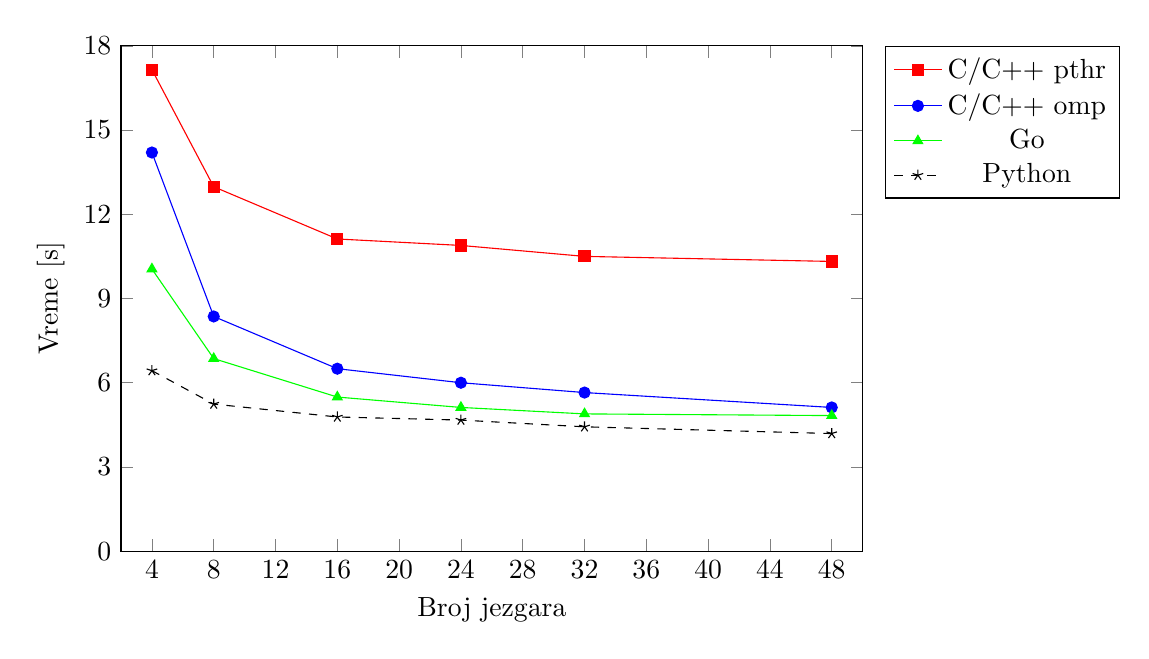
\begin{tikzpicture}
\begin{axis}[
    xlabel={Broj jezgara},
    ylabel={Vreme [s]},
    xmin=2, xmax=50,
    ymin=0, ymax=18,
    xtick={4,8,12,16,20,24,28,32,36,40,44,48},
    ytick={0,3,6,9,12,15,18},
    legend pos=outer north east,
    ymajorgrids=true,
    grid=none,
    width=11cm,
    height=8cm,
]

\addplot[red,mark=square* ]  coordinates {(4,17.15)(8,12.98)(16,11.12 )(24,10.89)(32,10.5)(48,10.32)}; 
\addplot[blue,mark=*]  coordinates {(4,14.2)(8,8.36)(16,6.5 )(24,6.0 )(32,5.65)(48,5.12)}; 
\addplot[green,mark=triangle*] coordinates {(4,10.05)(8,6.86)(16,5.49 )(24,5.12)(32,4.89)(48,4.83)};
\addplot[dashed,mark=star] coordinates {(4,6.43)(8,5.24)(16,4.78 )(24,4.67)(32,4.43)(48,4.19)};    
\legend{C/C++ pthr,C/C++ omp,Go,Python}
\end{axis}
\end{tikzpicture}

\caption{Grafik brzine izvršavanja različitih implementacija algoritma \textit{quicksort} u zavisnosti od broja jezgara, testirano za niz od $50\cdot10^{6}$  brojeva (osim Python-a koji je testiran za niz od $10^{6}$ brojeva)}
\label{fig:qs1}
\end{center}
\end{figure}

Maksimalna upotreba memorije za nizove različitih dužina prikazana je u tabeli \ref{tab:qs3}. Memorijski najefikasniji su C/C++ osim što pthreads verzija zahteva veliku količinu memorije za nizove manje dužine. Go koristi dva puta više memorije nego C/C++ omp, dok Python zahteva najviše memorije što je posledica upotrebljavanja procesa umesto niti. 

\begin{table}
\begin{center}
\caption{Maksimalna upotreba memorije [MB]  implementacija algoritma \textit{quicksort} za različite dužine niza}
\begin{tabular}{||c||c|c|c|c||}
\hline
\diagbox[width=2.7cm, height=1cm]{Verzija}{\vspace*{-0.8cm}n [$10^{6}$]} &1 &10 &30 &50 \\ \hline
C/C++ omp	& 9.2			&42.7			&121.5		&199.1	\\ 
C/C++ pthr	& 32.2		&76.9			&128.8		&229.3	\\ 
Go		& 11.3		&84.7			&245.5		&406.7	\\ 
Python	& 91.4		&827.9		& 2324.5		&3872.4	\\ \hline
\end{tabular}
\label{tab:qs3}
\end{center}
\end{table}

Dužine implementacija prikazane su u tabeli \ref{tab:qs4}.  Za implementaciju algoritma C/C++ pthreads verziji potreban je najveći broj linija koda, dok je u Python-u potreban najmanji.

\begin{table}
\begin{center}
\caption{Dužine kodova implementacija algoritma \textit{quicksort} }
\begin{tabular}{|c|c|c|c|c|c|c|}
\hline
		&  C/C++ pthr	& C/C++ omp & Go	& Python \\ \hline
Br. linija koda& 129	& 92	&84	&38	 \\ \hline
\end{tabular}
\label{tab:qs4}
\end{center}
\end{table}

\subsection{Rezime}

Za konkurentnu implementaciju algoritma \textit{quicksort}, Go se pokazao vremenski najefikasniji. Što se tiče memorijskih zahteva, Go koristi dva puta više memorije nego C/C++, ali je memorijski i vremenski višestruko efikasniji od Python-a. Dužina koda Go implementacije je manja od C/C++-a, ali znatno veća od Python-a. 

% Matrix==============================================================================

\section{Množenje matrica}
Za izradu implementacija upotrebljen je standardni algoritam za \textit{množenje matrica}. Vrednost na poziciji \textit{ij} proizvoda matrica A i B, izračunava se kao: $$(AB)_{ij} = \sum_{k=1}^{n} A_{ik}B_{kj}$$ gde su matrice A i B kvadratne matrice dimenzije \texttt{n}.

Algoritam je paralelizovan tako što svaka nit/gorutina računa po jedan red rezultujuće matrice, odnosno, jedan red prve matrice množi sa svim kolonama druge matrice. Za testiranje, korišćene su pseudoslučajno generisane kvadratne matrice različitih dimenzija. Kodovi svih implementacija dostupni su na repozitorijumu\footnote{\url{https://github.com/MitrovicMilosh/Go-Concurrency/tree/master/matrix_multiplication}}.

\subsection{Implementacija u jeziku Go}
Implementacija konkurentne funkcije za \textit{množenje matrica} prikazana je u primeru \ref{lst:matrix}. Broj gorutina koji se koristi prilikom izvršavanja algoritma zadaje se kao parametar funkcije. Gorutinama koje se kreiraju unutar \texttt{for} petlje neophodno je proslediti vrednost \texttt{i} kao parametar anonimne funkcije, kako bi svaka gorutina imala svoju kopiju. U suprotnom, u svakoj sledećoj iteraciji \texttt{for} petlje, vrednost \texttt{i} bi bila ažurirana u svim gorutinama. Za razliku od  implementacije \ref{lst:qs}, gde se niz koji se sortira prenosi pomoću reference, ovde su matrice definisane kao globalne. Nije potrebno nikakvo zaključavanje jer se ulazne matrice koriste samo za čitanje, a kod rezultujuće matrice svaka gorutina popunjava samo svoj red. 

\begin{center}
\begin{lstlisting}[caption=Implementacija konkurentne funkcije za \textit{množenje matrica} u jeziku Go,label={lst:matrix}, backgroundcolor=\color{background}]
func multiply_conc(num_routines int) {
	wg := sync.WaitGroup{}
	wg.Add(num_routines)
	for i := 0; i < num_routines; i++ {
		go func(row int){
			multiply_row(row, num_routines)
			wg.Done()
		}(i)
	}
	wg.Wait()
}
\end{lstlisting}
\end{center}

\subsection{Implementacije u drugim jezicima}
Implementacija u Python-u razlikuje se zbog nemogućnosti deljenja globalnih promenljivih, pa je matrice potrebno proslediti kao parametar funkcije, što ima negativan uticaj na memorijske zahteve. Paralelizacija implementacija u drugim jezicima, realizovana je na isti način. 

\subsection{Rezultati}

Grafik brzine konkurentnog izvršavanja u zavisnosti od veličine matrice, prikazan je na slici \ref{fig:matrix1}. Python se izvršava znatno sporije od ostalih implementacija, tako da nije bilo mogućnosti testirati ga za matrice iste veličine. Rezultati testiranja Python implementacije prikazani su u posebnim tabelama. Od prikazanih implementacija, C/C++ pthreads je vremenski najefikasnija. C/C++ omp i Go se izvršavaju istom brzinom za manje ulaze, ali za ulaze veće dimenzije Go radi dosta sporije. 

Grafik brzine sekvencijalnog izvršavanja u zavisnosti od veličine matrice prikazan je na slici \ref{fig:matrix11}. Sve implementacije dobijaju veliko ubrzanje konkurentnim izvršavanjem. Za matricu veličine 1500 implementacije rade duže od jednog minuta, dok im je pri konkurentnom izvršavanju potrebno od 3 do 10 sekundi.

\begin{figure}
\begin{center}

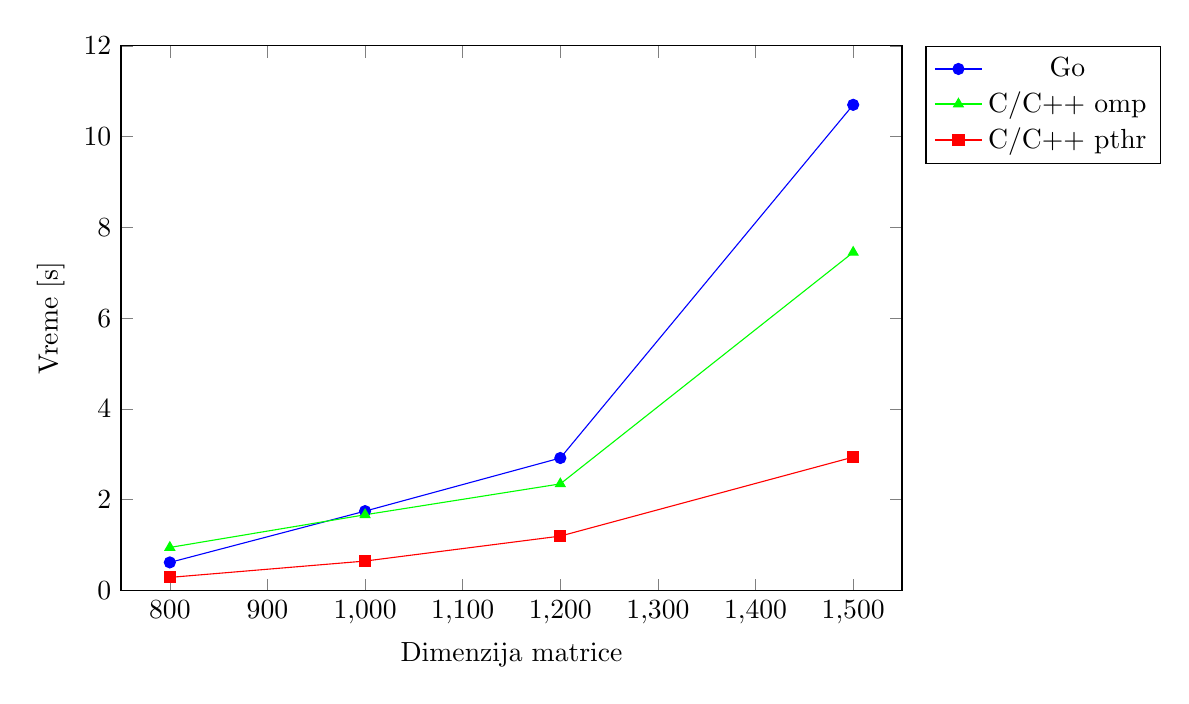
\begin{tikzpicture}
\begin{axis}[
    xlabel={Dimenzija matrice},
    ylabel={Vreme [s]},
    xmin=750, xmax=1550,
    ymin=0, ymax=12,
    xtick={800,900,1000,1100,1200,1300,1400,1500,1600},
    ytick={0,2,4,6,8,10,12},
    legend pos=outer north east,
    ymajorgrids=true,
    grid=none,
    width=11.5cm,
    height=8.5cm,
]

\addplot[blue,mark=*] coordinates {(800,0.62)(1000,1.75 )(1200,2.92)(1500, 10.7)}; 
\addplot[green,mark=triangle*] coordinates {(800,0.95 )(1000,1.67 )(1200,2.35)(1500,7.45 )}; 
\addplot[red,mark=square*] coordinates {(800,0.29)(1000,0.65)(1200,1.2)(1500,2.94 )}; 
\legend{Go, C/C++ omp, C/C++ pthr}
\end{axis}
\end{tikzpicture}

\caption{Grafik brzine konkurentnog izvršavanja različitih implementacija algoritma \textit{množenja matrica} u zavisnosti od veličine matrice, testirano na 48 jezgara}
\label{fig:matrix1}
\end{center}
\end{figure}

\begin{figure}
\begin{center}

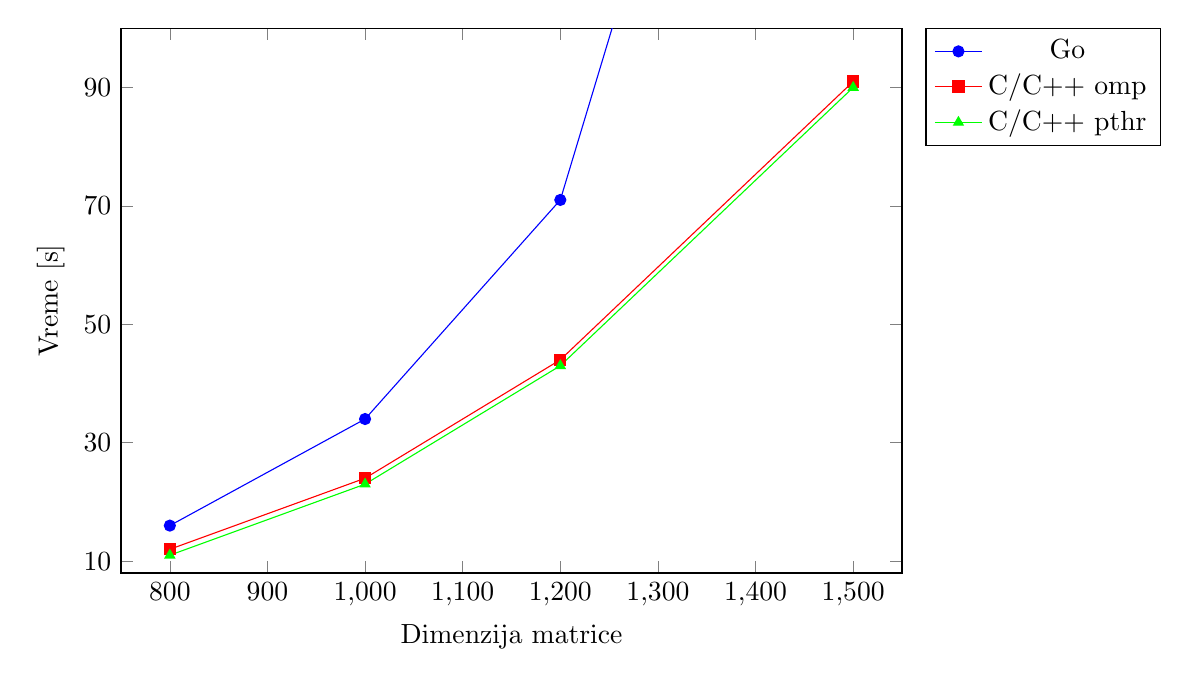
\begin{tikzpicture}
\begin{axis}[
    xlabel={Dimenzija matrice},
    ylabel={Vreme [s]},
    xmin=750, xmax=1550,
    ymin=8, ymax=100,
    xtick={800,900,1000,1100,1200,1300,1400,1500,1600},
    ytick={10,30,50,70,90},
    legend pos=outer north east,
    ymajorgrids=true,
    grid=none,
    width=11.5cm,
    height=8.5cm,
]

\addplot[blue,mark=*] coordinates {(800,16)(1000,34 )(1200,71)(1500,235)}; 
\addplot[red,mark=square*] coordinates {(800,12 )(1000,24)(1200,44)(1500,91 )}; 
\addplot[green,mark=triangle*] coordinates {(800,11)(1000,23)(1200,43)(1500,90 )}; 
\legend{Go, C/C++ omp, C/C++ pthr}
\end{axis}
\end{tikzpicture}

\caption{Grafik brzine sekvencijalnog izvršavanja različitih implementacija algoritma \textit{množenja matrica} u zavisnosti od veličine matrice}
\label{fig:matrix11}
\end{center}
\end{figure}

Prosečno vreme izvršavanja sa različitim brojem niti za matricu veličine 1000, prikazano je u tabeli \ref{tab:matrix5}. Implementacije postižu najbolje vreme sa 1000 niti/gorutina. Prilikom ostalih testiranja korišćen je onaj broj niti/gorutina za koji implementacija pokazuje najbolje rezultate, što je u ovom slučaju n niti/gorutina za matricu dimenzije n kod svih implementacija . 

\begin{table}
\begin{center}
\caption{Prosečno vreme izvršavanja [s] implementacija algoritma \textit{množenja matrica} sa različitim brojem niti, testirano sa 48 jezgara za matrice veličine 1000}
\begin{tabular}{||c||c c c c c||}
\hline
Br. niti		&40&100 &200 &500 &1000\\ \hline
C/C++ pthr	&1.48		&0.95		&0.85		&0.70		&\textbf{0.65} \\ \hline
C/C++ omp	&1.98		&1.81		&1.78		&1.71		&\textbf{1.67} \\ \hline
Go		&2.27		&2.16		&2.01		&1.84		&\textbf{1.75} \\ \hline
\end{tabular}
\label{tab:matrix5}
\end{center}
\end{table}

Rezultati testiranja implementacija na različitom broju jezgara prikazani su grafikom na slici \ref{fig:matrix3}. Implementacije dobijaju veliko ubrzanje povećanjem broja korišćenih jezgara. Ipak, ne postoji značajna razlika u brzini pri upotrebi 32 i 48 jezgara, što je posledica samog algoritma koji ne koristi dodatne optimizacije koje omogućavaju maksimalnu iskorišćenost procesora \cite{matp}.

\begin{figure}
\begin{center}

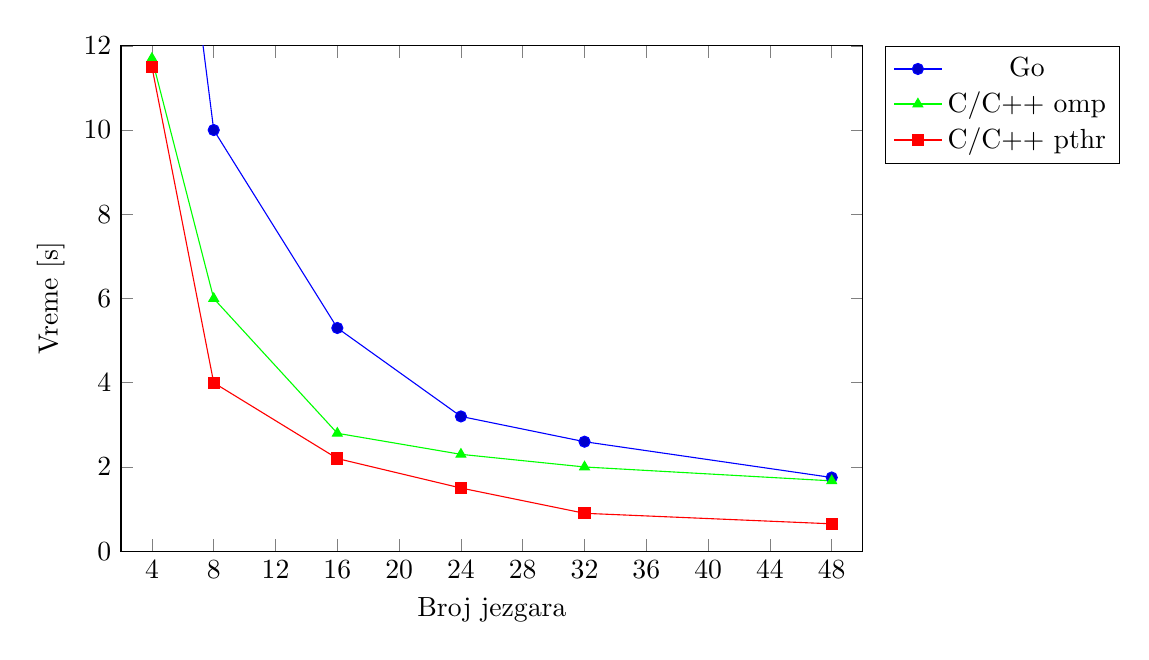
\begin{tikzpicture}
\begin{axis}[
    xlabel={Broj jezgara},
    ylabel={Vreme [s]},
    xmin=2, xmax=50,
    ymin=0, ymax=12,
    xtick={4,8,12,16,20,24,28,32,36,40,44,48},
    ytick={0,2,4,6,8,10,12},
    legend pos=outer north east,
    ymajorgrids=true,
    grid=none,
    width=11cm,
    height=8cm,
]
\addplot coordinates {(4,21.6)(8,10)(16,5.3)(24,3.2)(32,2.6)(48,1.75)}; 
\addplot[green,mark=triangle*]  coordinates {(4,11.7)(8,6)(16,2.8 )(24,2.3)(32,2.0)(48,1.67)}; 
\addplot[red,mark=square*] coordinates {(4,11.5)(8,4)(16,2.2 )(24,1.5 )(32,0.9)(48,0.65)}; 

\legend{Go, C/C++ omp, C/C++ pthr}
\end{axis}
\end{tikzpicture}

\caption{Grafik brzine izvršavanja različitih implementacija  algoritma \textit{množenja matrica} u zavisnosti od broja jezgara za matricu veličine 1000}
\label{fig:matrix3}
\end{center}
\end{figure}

Grafik maksimalne upotrebe memorije u zavisnosti od dimenzije matrice prikazan je na slici \ref{fig:matrix2}. Implementacije imaju slične memorijske zahteve, osim što za veće ulaze Go zahteva nešto više memorije od ostalih.

\begin{figure}
\begin{center}

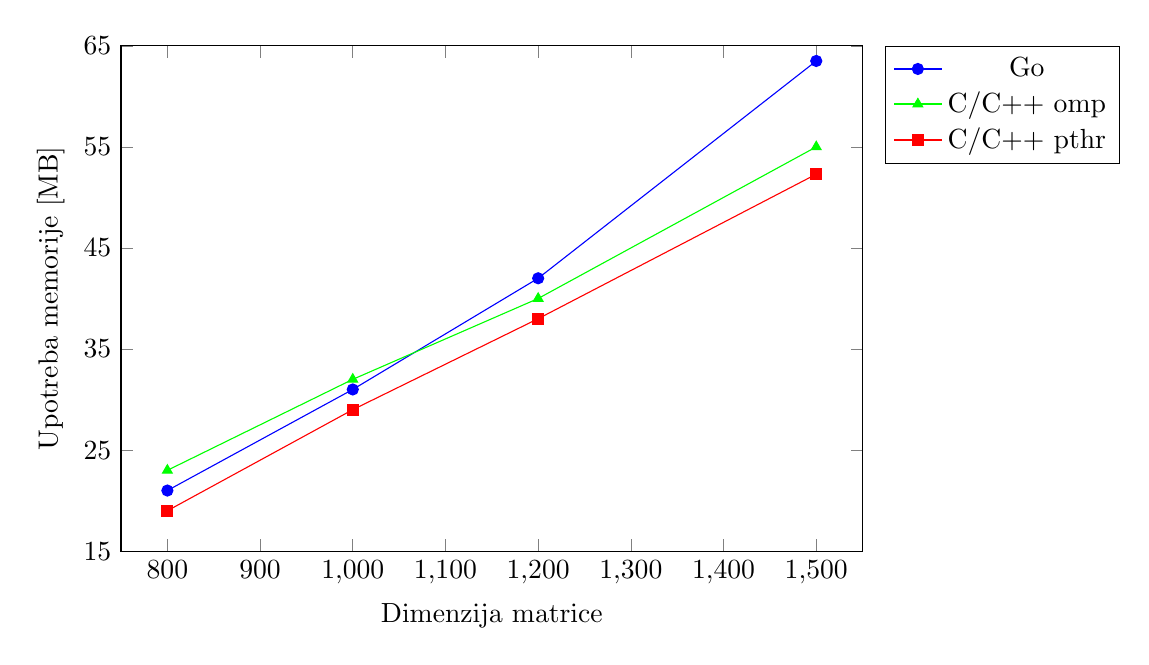
\begin{tikzpicture}
\begin{axis}[
    xlabel={Dimenzija matrice},
    ylabel={Upotreba memorije [MB]},
    xmin=750, xmax=1550,
    ymin=15, ymax=65,
    xtick={800,900,1000,1100,1200,1300,1400,1500},
    ytick={15,25,35,45,55,65},
    legend pos=outer north east,
    ymajorgrids=true,
    grid=none,
    width=11cm,
    height=8cm,
]
\addplot[blue,mark=*] coordinates {(800,21)(1000,31 )(1200,42)(1500,63.5)}; 
\addplot[green,mark=triangle*] coordinates {(800,23)(1000,32)(1200,40)(1500,55 )}; 
\addplot[red,mark=square*] coordinates {(800,19 )(1000,29)(1200,38)(1500,52.3)}; 
\legend{Go, C/C++ omp, C/C++ pthr}
\end{axis}
\end{tikzpicture}

\caption{Grafik maksimalne upotrebe memorije  u zavisnosti od dimenzije matrica, različitih implementacija algortima \textit{množenja matrica}}
\label{fig:matrix2}
\end{center}
\end{figure}

Rezultati Python implementacije prikazani su u tabeli \ref{tab:matrix1}. Python radi višestruko sporije od ostalih implementacija. Za matricu veličine 800, potrebno mu je više od 3 minuta, dok ostale implementacije rade ispod jedne sekunde. U odnosu na sekvencijalno izvršavanje Python se izvršava oko tri puta brže. Kada je reč o memorijskim zahtrevima pri konkurentnom izvršavanju, Python-u je potrebna pet puta veća količina memorije nego ostalim implementacijama, što je posledica upotrebe procesa umesto niti.

U  tabeli \ref{tab:matrix11} prikazano je vreme izvršavanja u zavisnosti od broja jezgara Python implementacije, za matricu veličine 300. Kod Python-a, sa povećanjem broja jezgara ne dobija se značajno ubrzanje za razliku od drugih jezika. 

U  tabeli \ref{tab:matrix111} prikazano je vreme izvršavanja sa različitim brojem niti u zavisnosti od broja jezgara Python implementacije, za matricu veličine 300. Broj niti, kao i broj jezgara  nema značajan uticaj na brzinu izvršavanja kod Python-a.

\begin{table}
\begin{center}
\caption{Prosečno vreme izvršavanja i maksimalna upotreba memorije pri konkurentnom izvršavanju za različito n,  implementacije  algoritma \textit{množenja matrica}  u jeziku Python}
\begin{tabular}{||c||c|c|c||}
\hline
n & Konkurentno [s]& Sekvencijalno [s] & Memorija [MB] \\ \hline
100	&0.55		&1.41		&15.5\\
300	&10.78	&25.54	&22.7\\
500	&51.19	&144.52	&47.8\\
800	&195.293	&- 		&115.3\\
\hline
\end{tabular}
\label{tab:matrix1}
\end{center}
\end{table}

\begin{table}
\begin{center}
\caption{Prosečno vreme izvršavanja u zavisnosti od broja jezgara za matricu veličine 300, implementacije algoritma \textit{množenja matrica} u jeziku Python}
\begin{tabular}{||c||c|c|c|c|c|c||}
\hline
Br. jezgara &4  &8 &16 &24 & 32 &48 \\ \hline
Vreme [s]	&14.70	&12.84	&11.66 	& 10.91	&10.85	&10.78\\ \hline  
\end{tabular}
\label{tab:matrix11}
\end{center}
\end{table}

\begin{table}
\begin{center}
\caption{Prosečno vreme izvršavanja sa različitim brojem niti  za matricu veličine 300, implementacije algoritma \textit{množenja matrica} u jeziku Python}
\begin{tabular}{||c||c|c|c|c|c|c||}
\hline
Br. niti &4 &10 &30 &50 &100 & 300  \\ \hline
Vreme [s]	&12.57	&11.60	&10.91	 & 10.82	&10.85	&10.78\\ \hline
\end{tabular}
\label{tab:matrix111}
\end{center}
\end{table}

Broj linija koda svih  implementacija prikazan je u tabeli \ref{tab:matrix2}. Najdužu implementaciju algoritma ima C/C++ pthreads, dok najkraću ima Python.

\begin{table}
\begin{center}
\caption{Dužine kodova implementacija množenja matrica}
\begin{tabular}{|c|c|c|c|c|c|}
\hline
		&  C/C++ pthr 	& Go	& C/C++ omp	& Python	\\ \hline
Br. linija koda& 78	& 71	&55		&28		\\ \hline
\end{tabular}
\label{tab:matrix2}
\end{center}
\end{table}

\subsection{Rezime}

Za konkurentnu implementaciju algoritma \textit{množenja matrica}, Go se pokazao vremenski efikasan koliko i C/C++ za ulaze manjih dimenzija, dok za ulaze većih dimenzija zahteva više vremena. Go upotrebljava nešto više memorije nego C/C++ za matrice većih dimenzija, ali je neuporedivo vremenski i memorijski efikasniji od Python-a. Potreban je približno isti broj linija koda za implementaciju algoritma u Go-u kao i za C/C++ pthreads verziju.

% Prime==============================================================================

\section{Eratostenovo sito} \label{erathost}
Eratostenovo sito je algoritam za određivanje prostih brojeva manjih od n. Ideja algoritma je da se eliminišu svi brojevi koji nisu prosti između 2 i \texttt{n}. Na početku se pretpostavlja da su svi brojevi prosti, odnosno definiše se niz od \texttt{n} bulovskih vrednosti postavljenih na \texttt{true}. Polazi se od prvog prostog broja što je 2, i eliminišu se brojevi deljivi sa 2, odnosno za svaki drugi broj odgovarajuća bulovska promenljiva se postavlja na \texttt{false} počevši od $2^{2}$, a zatim, prelazi se na sledeći prost broj i postupak se ponavlja. Uopšteno, za prost broj \texttt{i} eliminiše se svaki i-ti broj počevši od  $\texttt{i}^{2}$. Postupak je dovoljno ponoviti za proste brojeve koji su manji od $\sqrt{\texttt{n}}$. Pseudokod algoritma je prikazan na slici \ref{fig:prime_pseudo}.

\begin{figure}
\begin{center}

\begin{Verbatim}[fontsize=\small]
for i:=2 to n do
    A[i]:=true

ErathostenesSieve(n):
    for i:=2 to floor(sqrt(n)) do 
         if A[i] = true:
             j := i * i
             while j < n do
                 A[j] := false 
                 j := j + i
\end{Verbatim}

\caption{Pseudokod algoritma \textit{Eratostenovo sito}}
\label{fig:prime_pseudo}
\end{center}
\end{figure}

Paralelizacija algoritma se postiže deljenjem opsega od 2 do \texttt{n} na jednake delove. Svaka nit/gorutina dobija svoj deo opsega u okviru kojeg eliminiše brojeve koji nisu prosti. Za svaki prost broj prvo je potrebno odrediti njegov prvi umnožak unutar opsega. Iako svaka nit/gorutina ima svoj opseg, ona mora da pristupa članovima niza drugih niti/gorutina jer su joj potrebni svi prosti brojevi manji od $\sqrt{\texttt{n}}$. To kao posledicu dovodi do mogućnosti da se u nekim slučajevima bespotrebno eliminišu umnošci brojeva koji nisu prosti ukoliko ih druga nit/gorutina još uvek nije eliminisala. Problem je rešen tako što se proverava dodatni uslov prilikom eliminacije: da li je neka druga nit/gorutina u međuvremenu označila da taj broj nije prost. Kodovi svih implementacija, dostupni su na repozitorijumu\footnote{\url{https://github.com/MitrovicMilosh/Go-Concurrency/tree/master/prime_sieve}}.

\begin{center}
\begin{lstlisting}[caption=Implementacija konkurentne funkcije za određivanje prostih brojeva manjih od n u jeziku Go,label={lst:prime1},backgroundcolor=\color{background}]
func Prime(list *[]bool, n int, is_concurrent bool){
	sqrt := int(math.Sqrt(float64(n)))
	first := 0
	step := int(n/ num_goroutines)
	last := step
	wg := sync.WaitGroup{}
	wg.Add(num_goroutines)

	for i:=0; i < num_goroutines-1; i++{
		go mark_prime(list,first,last,sqrt,&wg,true)
		first = last + 1
		last += step
	}

	mark_prime(list,first,n-1,sqrt,&wg)
	wg.Wait()
}
\end{lstlisting}
\end{center}

\subsection{Implementacija u jeziku Go}
Funkcija koja kreira gorutine prikazana je u primeru \ref{lst:prime1}. Za svaki broj koji je trenutno označen kao prost najpre je potrebno odrediti njegov prvi umnožak, a zatim označiti sve njegove umnoške unutar opsega što je i prikazano u primeru \ref{lst:prime2}. Koristi se globalni niz od \texttt{n} bulovskih promenljivih postavljenih na podrazumevanu vrednost \texttt{false} umesto na \texttt{true} radi jednostavnosti. Kao što je već pomenuto, ako svaka gorutina ima svoj opseg, ona mora da pristupa i članovima niza drugih gorutina jer su joj potrebni svi prosti brojevi manji od $\sqrt{\texttt{n}}$. To kao posledicu dovodi do pojave trke za resursima, međutim u ovom slučaju je to dopustivo i nisu potrebni muteksi, upravo zato što se proverava dodatni uslov da li je pročitana vrednost u međuvremenu bila menjana. Ako se detektor trke za resursima pozove, dobija se izveštaj koji upozorava da je ona prisutna. Primer izveštaja se može videti u poglavlju \ref{datarace} na slici \ref{fig:datarace}. 

\begin{center}
\begin{lstlisting}[caption=Implementacija konkurentne funkcije za označavanje prostih brojeva u jeziku Go,label={lst:prime2}, backgroundcolor=\color{background}]
func mark_prime(list *[]bool,first,last,sqrt int,wg *sync.WaitGroup){
	for i:=2;  i<= sqrt && i*i<= last; i++{
		if !(*list)[i] {
			var j int
			if i*i < first {
				if (first - i*i)%i == 0 {
					j = i*i + ((first-i*i)/i)*i
				}else {
					j = i*i + ((first-i*i)/i + 1)*i
				}
			}else {
				j = i*i
			}
		
			for ; j <= last && !(*list)[i]; j+=i {
				(*list)[j] = true
			}
		}
	}
	wg.Done()
}
\end{lstlisting}
\end{center}

\subsection{Ostale implementacije}
Implementacija u Python-u razlikuje se zbog nemogućnosti deljenja globalnih promenljivih, pa je odgovarajući deo niza potrebno proslediti kao parametar funkcije, što ima uticaj na memorijske zahteve. Na ovaj način je onemogućena provera toga da li se eliminišu umnošci broja koji je već označen da nije prost, što ima uticaj na vremensku efikasnost. Implementacije u ostalim jezicima realizovane su na isti način.

\subsection{Rezultati}

Prosečno vreme konkurentnog i sekvencijalnog izvršavanja implementacija predstavljeno je grafikom na slici \ref{fig:prime1}. Python nije mogao da bude uključen na ovom grafiku usled znatno sporijeg izvršavanja, a rezultati Python implementacije prikazani su u posebnim tabelama. Go i C/C++ omp su vremenski najefikasniji i povećanje vrednosti n ne utiče značajno na njihovo vreme izvršavanja. U odnosu na sekvencijalno izvršavanje sve implementacije dobijaju višestruko ubrzanje. 

\pgfplotsset{ every non boxed x axis/.style={} }

\begin{figure}
\begin{center}

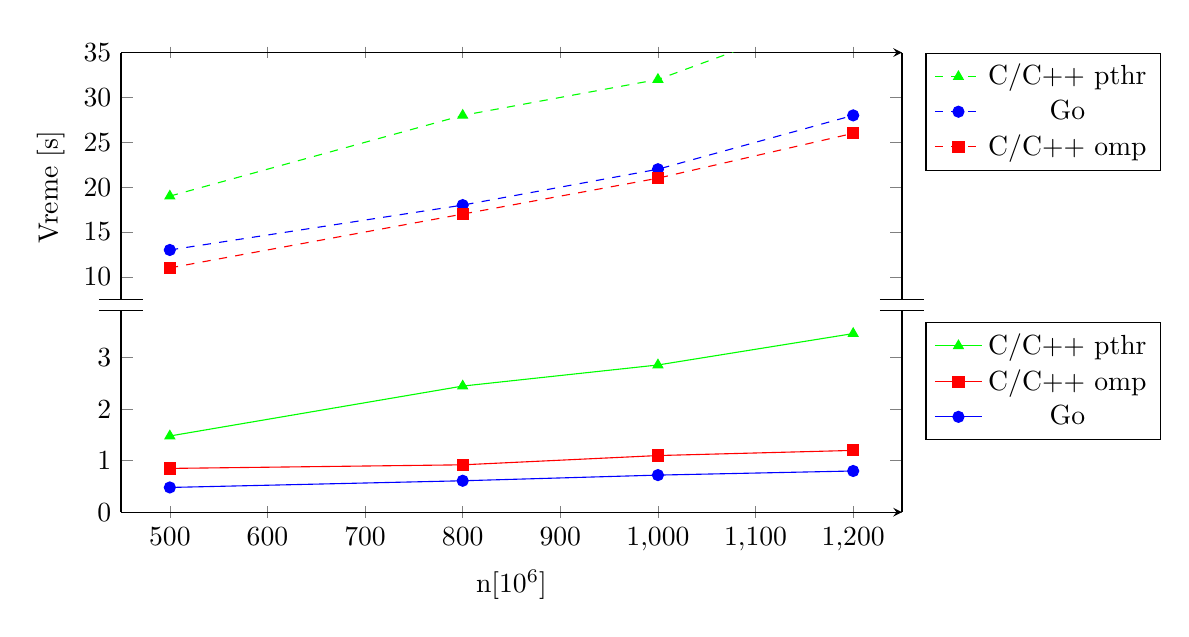
\begin{tikzpicture}
\begin{groupplot}[
    group style={
        group name=my fancy plots,
        group size=1 by 2,
        xticklabels at=edge bottom,
        vertical sep=0cm
    },
    xlabel={n[$10^{6}$]},
    ylabel={Vreme [s]},
    xmin=450, xmax=1250,
    xtick={500,600,700,800,900,1000,1100,1200},
    legend pos=outer north east,
    ymajorgrids=true,
    grid=none,
    width=11.5cm,
]


\nextgroupplot[ymin=5,ymax=35,
               ytick={10,15,20,25,30,35},
               axis x line=top, 
               axis y discontinuity=parallel,
               height=5.0cm,
	    xlabel={}]

\addplot[green,  mark=triangle*, dashed,mark options={solid}] coordinates {(500,19)(800,28)(1000, 32)(1200, 40)};
\addplot[blue, dashed, mark=*,mark options={solid}] coordinates {(500,13)(800,18 )(1000, 22)(1200, 28)};   
\addplot[red, dashed, mark=square*,mark options={solid}] coordinates {(500,11)(800,17)(1000, 21)(1200, 26)};
\legend{C/C++ pthr,Go,C/C++ omp}


\nextgroupplot[ymin=0,ymax=3.7,
               ytick={0,1,2,3},
               axis x line=bottom,
               height=4.0cm, ylabel={}]

\addplot[green,mark=triangle*] coordinates {(500, 1.48)(800,2.45 )(1000,2.86 )(1200, 3.47)}; 
\addplot[red,mark=square*] coordinates {(500,0.85 )(800,0.92 )(1000,1.1)(1200, 1.2)}; 
\addplot[blue,mark=*] coordinates {(500,0.48 )(800,0.61)(1000, 0.72)(1200, 0.8)}; 
\legend{C/C++ pthr,C/C++ omp,Go}

\end{groupplot}
\end{tikzpicture}
\caption{Grafik brzine izvršavanja različitih implementacija algoritma \textit{Eratostenovo sito} za različito n, testirano na 48 jezgara; isprekidanom linjom, prikazano je sekvencijalno izvršavanje dok je konkurentno prikazano punom linijom}
\label{fig:prime1}

\end{center}
\end{figure}

U tabeli \ref{tab:prime5} prikazano je vreme izvršavanja sa različitim brojem niti/gorutina kada n iznosi $1000\cdot10^{6}$. Sve tri implementacije postižu najbolje performanse sa 10000 niti/gorutina. Broj niti/gorutina utiče na opseg pretraživanja i veličinu posla koju jedna nit/gorutina obavlja, što ima velike posledice na vremensku efikasnost.

\begin{table}
\begin{center}
\caption{Prosečno vreme izvršavanja [s] implementacija algoritma \textit{Eratostenovo sito} sa različitim brojem niti, testirano sa 48 jezgara kada n iznosi $1000\cdot10^{6}$}
\begin{tabular}{||c||c c c c c||}
\hline
Br. niti		&50 &100 &1000 &10000&100000\\ \hline
Go		&4.15	&3.21	&0.78&\textbf{0.71}&1.31\\ \hline
C/C++ omp  &14.53&9.84	&5.31&\textbf{1.12}&1.41\\ \hline
C/C++ pthr	&7.34	&6.13	&5.02&\textbf{2.62}&4.72\\ \hline
\end{tabular}
\label{tab:prime5}
\end{center}
\end{table}

Grafik brzine izvršavanja implementacija u zavisnosti od broja jezgara prikazan je na slici \ref{fig:prime3}. Kod svih implementacija postoji ubrzanje sa povećanjem broja jezgara, ali ne postoji značajna razlika u brzini prilikom izvršavanja sa 32  i 48 jezgara, što je posledica ograničenja samog algoritma bez optimizacije.

\begin{figure}
\begin{center}

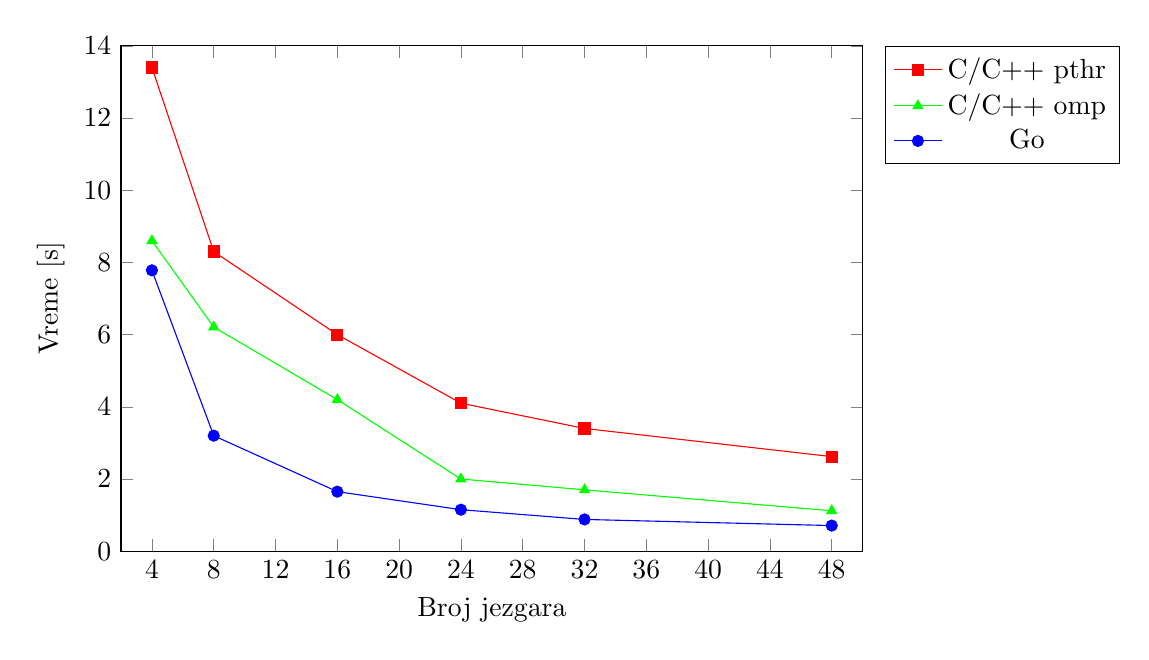
\begin{tikzpicture}
\begin{axis}[
    xlabel={Broj jezgara},
    ylabel={Vreme [s]},
    xmin=2, xmax=50,
    ymin=0, ymax=14,
    xtick={4,8,12,16,20,24,28,32,36,40,44,48},
    ytick={0,2,4,6,8,10,12,14},
    legend pos=outer north east,
    ymajorgrids=true,
    grid=none,
    width=11cm,
    height=8cm,
]
\addplot[red,mark=square* ]   coordinates {(4,13.4)(8,8.3)(16,6 )(24,4.1 )(32,3.4)(48,2.62)}; 
\addplot[green,mark=triangle*] coordinates {(4,8.60)(8,6.21)(16,4.2 )(24,2)(32,1.7 )(48,1.12)}; 
\addplot[blue,mark=*] coordinates {(4,7.78)(8,3.2)(16,1.65)(24,1.15 )(32,0.88 )(48,0.71)}; 
\legend{C/C++ pthr,C/C++ omp,Go}
\end{axis}
\end{tikzpicture}

\caption{Grafik brzine izvršavanja različitih implementacija algoritma \textit{Eratostenovo sito} u zavisnosti od broja jezgara  kada n iznosi 1 milijaradu}
\label{fig:prime3}
\end{center}
\end{figure}


Maksimalna upotreba memorije u zavisnosti od n prikazana je grafikom na slici \ref{fig:prime2}. Sve tri implementacije imaju slične memorijske zahteve. Na grafiku se vidi približno linearna zavisnost y=x, što znači da je potrebna količina memorije direktno proporcijalna vrednosti n.

Prosečno vreme izvršavanja i upotreba memorije Python implementacije pri konkurentnom izvršavanju, prikazani su u tabeli \ref{tab:prime1}. Python radi najsporije od svih implementacija i potrebno mu je više od 20 sekundi za ulaz veličine $10\cdot10^{6}$, dok ostale implementacije rade oko jedne sekunde za ulaz veličine $500\cdot10^{6}$. U odnosu na sekvencijalno izvršavanje Python dobija ubrzanje koje je neuporedivo manje u odnosu na druge jezike. Memorijski zahtevi su takođe znatno veći u odnosu na druge implementacije usled upotrebe procesa umesto niti.

\begin{figure}[H]
\begin{center}

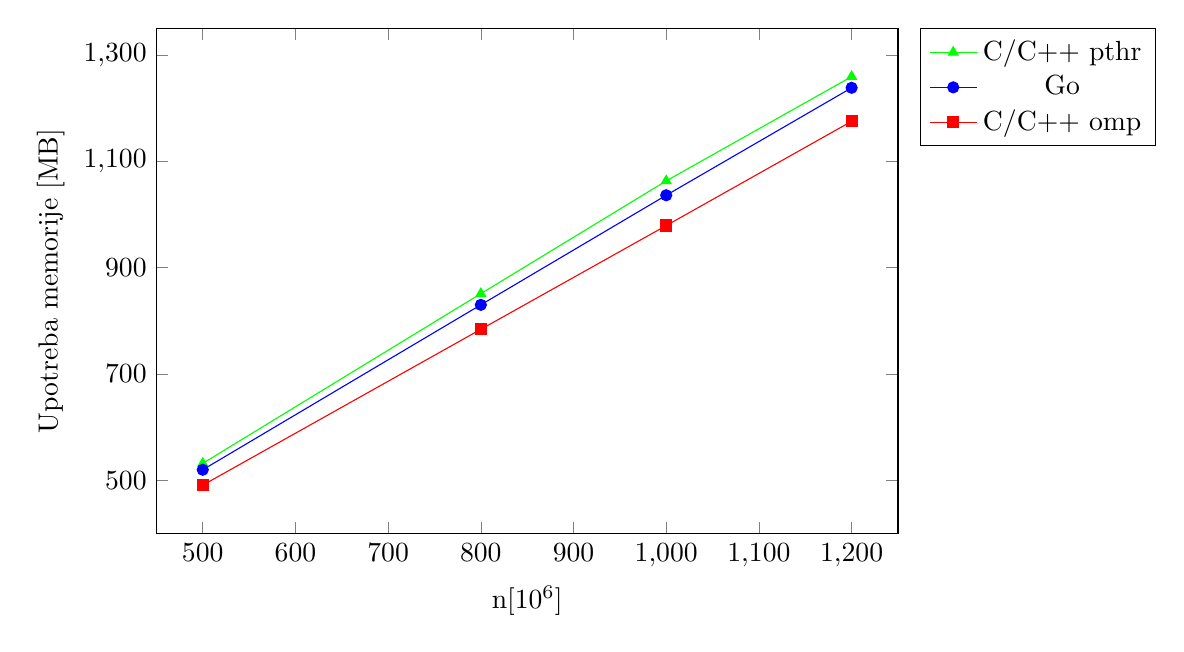
\begin{tikzpicture}
\begin{axis}[
    xlabel={n[$10^{6}$]},
    ylabel={Upotreba memorije [MB]},
    xmin=450, xmax=1250,
    ymin=400, ymax=1350,
    xtick={500,600,700,800,900,1000,1100,1200},
    ytick={500,700,900,1100,1300},
    legend pos=outer north east,
    ymajorgrids=true,
    grid=none,
    width=11cm,
    height=8cm,
]
\addplot[green,mark=triangle*] coordinates {(500,532 )(800,851 )(1000,1063)(1200, 1259)}; 
\addplot[blue,mark=*] coordinates {(500, 520)(800,830 )(1000,1036 )(1200, 1238)}; 
\addplot[red,mark=square*] coordinates {(500,491 )(800,784)(1000,979)(1200, 1175)}; 
\legend{C/C++ pthr,Go,C/C++ omp}
\end{axis}
\end{tikzpicture}

\caption{Grafik maksimalne upotrebe memorije različitih implementacija algoritma \textit{Eratostenovo sito} za različito n}
\label{fig:prime2}
\end{center}
\end{figure}

\begin{table}[H]
\begin{center}
\caption{Prosečno vreme izvršavanja i maksimalna upotreba memorije pri konkurentnom izvršavanju za različito n, implementacije algoritma \textit{Eratostenovo sito} u jeziku Python}
\begin{tabular}{||c||c|c|c||}
\hline
n & Konkurentno [s]& Sekvencijalno [s] & Memorija [MB] \\ \hline
100,000	&0.12	&0.19&17.2\\
1,000,000	&1.95	&3.15&102.4\\
10,000,000	&23.88&29.63&888.7\\
\hline
\end{tabular}
\label{tab:prime1}
\end{center}
\end{table}

\begin{table}[H]
\begin{center}
\caption{Prosečno vreme izvršavanja  u zavisnosti od broja jezgara za n = $10^{6}$, implementacije algoritma \textit{Eratostenovo sito} u jeziku Python}
\begin{tabular}{||c||c|c|c|c|c|c||}
\hline
Br. jezgara &4  &8 &16 &24 & 32 &48 \\ \hline
Vreme [s]	&2.93		&2.42		&2.13 	& 2.01	&1.96 	&1.95\\ \hline  
\end{tabular}
\label{tab:prime11}
\end{center}
\end{table}

\begin{table}[H]
\begin{center}
\caption{Prosečno vreme izvršavanja  sa različitim brojem niti za n = $10^{6}$, implementacije algoritma \textit{Eratostenovo sito} u jeziku Python}
\begin{tabular}{||c||c|c|c|c|c|c||}
\hline
Br. niti &4 &10 &30 &50 &100 & 500  \\ \hline
Vreme [s]	&2.38		&2.03		&2.05	 	& 1.98	&1.95		&2.07\\ \hline
\end{tabular}
\label{tab:prime111}
\end{center}
\end{table}

U  tabeli \ref{tab:prime11} prikazano je vreme izvršavanja u zavisnosti od broja jezgara, a u tabeli \ref{tab:prime111} vreme izvršavanja sa različitim brojem niti, za Python implementaciju kada n iznosi $10^{6}$. Povećanje broja jezgara nema značajan uticaj na vremensku efikasnost Pythona, kao ni različit broj niti koji se koristi.

Dužine implementacija su prikazane u tabeli \ref{tab:prime2}. Najkraća implementacija algoritma je u Python-u, dok je najduža C/C++ pthreads verzija.

\begin{table}[H]
\begin{center}
\caption{Dužine kodova implementacija algoritma \textit{Eratostenovo sito}}
\begin{tabular}{|c|c|c|c|c|}
\hline
		&  C/C++ pthr	&Go 	& C/C++ omp & Python 	 \\ \hline
Br. linija koda&98		& 82	&70	&42		 \\ \hline
\end{tabular}
\label{tab:prime2}
\end{center}
\end{table}


\subsection{Rezime}

Za implementaciju algoritma \textit{Eratostenovo sito}, Go se ispostavio kao vremenski najefikasniji sa značajnim ubrzanjem u odnosu na sekvencijalno izvršavanje. Go ima približno istu upotrebu memorije kao C/C++, kao i približno istu dužinu implementacije.

%Aplikacija================================================================

\chapter{Primer upotrebe programskog jezika Go}\label{app}

Kao primer upotrebe programskog jezika Go razvijena je serverska aplikacija\ koja demonstrira korišćenje konkurentnosti kao i drugih aspekata jezika. U ovoj glavi predstavljena je struktura aplikacije i opisani su pojedinačni delovi koji ilustruju različite karakteristike programskog jezika. 

\section{Serverska aplikacija}

Razvijena serverska aplikacija se bavi primenom različitih filtera na slikama. Omogućava primenu postojećih predefinisanih filtera kao i kreiranje sopstvenog, kombinovanjem različitih ponuđenih filtera i unošenjem željenih vrednosti za pojedine karakteristike. Slika koje se obrađuje se može učitati sa računara ili se može proslediti njen URL. Svi filteri se primenjuju paralelno nakon čega se mogu videti pojedinačni rezultati obrade koji su dostupni za preuzimanje. Kompletan kod aplikacije je dostupan na repozitorijumu\footnote{\url{https://github.com/MitrovicMilosh/Go-Concurrency/blob/master/server/server.go}}. Za razvoj korišćena je Go 1.8 verzija programskog jezika. Grafički interfejs aplikacije je prikazan na slici \ref{fig:interface}.

\begin{figure}
\begin{center}
\includegraphics[scale=1.4]{interface.png}
\end{center}
\caption{Grafički interfejs početne stranice i stranice za prikaz rezultata serverske aplikacije za primenu filtera}
\label{fig:interface}
\end{figure}

\subsection{Struktura aplikacije}
Struktura aplikacije predstavljena je dijagramom na slici \ref{fig:diag}. Server, na osnovu zahteva koji dobija od korisnika, poziva odgovarajuću funkciju za rukovanje (engl. "handler"). Definisane su dve funkcije za rukovanje: \texttt{DefaultHandle} koja ima zadatak da generiše početnu HTML stranicu, i \texttt{ImageHandler} koja se bavi preuzimanjem i obradom datoteka, primenom filtera na slici i generisanjem HTML stranice za prikaz rezultata. 
 
\begin{figure}
\begin{center}
\includegraphics[scale=0.45]{dijagram.png}
\end{center}
\caption{Dijagram koji prikazuje strukturu aplikacije}
\label{fig:diag}
\end{figure}

\subsection{Kreiranje servera i obrada zahteva}

Za kreiranje servera je korišćen paket \texttt{net/http} koji obezbeđuje skup funkcija za jednostavnu implementaciju i upravljanje serverom. Jednostavni server prikazan je u primeru \ref{lst:server1}. 

\begin{center}
\begin{lstlisting}[caption=Jednostavni server,label={lst:server1},   backgroundcolor=\color{background}]
package main
import ("net/http"; "fmt")

func hello(w http.ResponseWriter, r *http.Request) {
	fmt.Fprintln(w,"Hello!")
}
func main() {
	http.HandleFunc("/", hello)
	http.ListenAndServe(":12345", nil)
}
\end{lstlisting}
\end{center}


Funkcija \texttt{HandleFunc} se koristi za registrovanje funkcija za rukovanje za određeni šablon. Funkcija za rukovanje kao parametre ima \texttt{ResponseWriter} koji se koristi za konstrukciju HTTP odgovora i \texttt{Request} koji sadrži sve podatke HTTP zahteva. Funkcija \texttt{ListenAndServe} osluškuje na zadatoj adresi (prvi parametar) TCP mreže i poziva funkciju \texttt{Serve} kojoj prosleđuje promenljivu tipa \texttt{Handler} (drugi parametar). U pozadini, funkcija \texttt{Serve} kreira novu gorutinu za svaku HTTP konekciju i poziva funkciju za rukovanje. Ukoliko je promenljiva tipa \texttt{Handler} \texttt{nil}, koristi se multiplekser \texttt{DefaultServeMux} koji uparuje URL zahteve sa registrovanim šablonima i poziva odgovarajuću funkciju za rukovanje\cite{http}.

Server se može implementirati u Go-u  koristeći samo dva paketa i manje od deset linija koda što je karakteristično za dinamički tipizirane, interpretirane jezike kao što su Python, PHP, Ruby i drugi. U C/C++ -u, koji su statički tipizirani jezici koji se kompiliraju, kao što je i Go, je potrebno devet bibiloteka i više od pedeset linija koda \cite{server}.

Deo koda koji se odnosi na kreiranje servera u aplikaciji nalazi se u funkciji \texttt{main} koja je prikazana u primeru \ref{lst:main}. Funkcijom \texttt{HandleFunc} registrovane su dve funkcije za rukovanje: \texttt{DefaultHandler} koja se poziva kada se pristupa početnoj strani i \texttt{ImageHandler} koja se poziva prilikom obrade slike i prikazivanja rezultata. Funkcija \texttt{Handle} koristi se za registrovanje funkcije za rukovanje sa sistemom datoteka i šablona koji se odnosi na zahteve resursa.  U funkciji \texttt{ListenAndServe} je postavljeno da se osluškuje na http portu zadate adrese servera koja je u ovom slučaju postavljena na \texttt{localhost}.

\begin{center}
\begin{lstlisting}[caption={Funkcija \texttt{main}, kreiranje servera},label={lst:main},  backgroundcolor=\color{background} ]
func main() {
	fmt.Println("Starting server...")
	rand.Seed(time.Now().UTC().UnixNano())
	http.HandleFunc("/", DefaultHandler)
	http.HandleFunc("/results", ImageHandler)
	http.Handle("/data/", http.HandlerFunc(file_server))
	http.ListenAndServe(address + ":http", nil)
}
\end{lstlisting}
\end{center}

\label{fileserver}Funkcija za rukovanje sa sistemom datoteka prikazana je u primeru \ref{lst:fileserver}. U ovoj funkciji definišu se restrikcije nad URL zahtevima za resurse i definiše se korenog direktorijum svih resursa. URL se deli na segmente funkcijom split i zatim se ispituje poslednji segment. Ukoliko je poslednji segment prazan odnosno ako se URL završava znakom \texttt{/}, to znači da u zahtevu nije tražena određena datoteka već je u pitanju samo deo putanje. \texttt{DefaultServeMux} funkcioniše tako što dodaje znak \texttt{/} na kraju svakog URL zahteva koji postoji u podstablu root direktorijuma, što znači da ako korisnik unese putanju do nekog direktorijuma, poslednji deo URL zahteva će biti prazan \cite{http}. U tom slučaju korisniku će biti onemogućen pristup direktorijumu i neće moći da pročita njegov sadržaj.

\begin{center}
\begin{lstlisting}[caption=Funkcija za rukovanje sa sistemom datoteka,label={lst:fileserver},  backgroundcolor=\color{background}]
func file_server(w http.ResponseWriter, r *http.Request) {
	parts := strings.Split(r.URL.Path, "/")
	last := parts[len(parts)-1]
	if last == "" {
		http.NotFound(w, r)
		return
	}
	fileServer := http.StripPrefix("/data/", 
				http.FileServer(http.Dir("data"))).ServeHTTP(w, r)
}
\end{lstlisting}
\end{center}

\subsection{Generisanje HTML stranice}

Paket \texttt{html/template} koristi se za generisanje HTML izlaza sa datim parametrima koji ima zaštitu protiv umetanja koda. Paket nudi veliki broj različitih escape funkcija koje kodiraju specijalne karaktere, ali u ovoj aplikaciji nije bilo potrebe za njihovom upotrebom. 

\begin{center}
\begin{lstlisting}[caption=Izvršavanje HTML šablona,label={lst:tmpl},  backgroundcolor=\color{background}]
func DefaultHandler(w http.ResponseWriter, r *http.Request) {
	...
	tmpl, _ := template.ParseFiles("index.html")
	tmpl.ExecuteTemplate(w, "index", data)
}
\end{lstlisting}
\end{center}

U funkciji \texttt{DefaultHandler} parsira se i izvršava šablon koji se prikazuje kada se pristupi početnoj strani. Deo funkcije koji se odnosi na izvršavanje šablona je prikazan u primeru \ref{lst:tmpl}. Ovde, kao i na drugim mestima, moguće greške će biti ignorisane jer se podrazumeva da su parametri funkcije ispravni i da neće doći do greške. Fiksni parametri su provereni tokom faze razvijanja i debagovanja aplikacije, dok parametri koji zavise od unosa korisnika, prethodno prolaze kroz odgovarajuće provere. Funkcija \texttt{ExecuteTemplate} kao argumente prima \texttt{ResponseWriter}, naziv šablona koji se izvršava i podatke koji se koriste za njegovo popunjavanje. Prosleđena promenljiva \texttt{data} je definisana struktura koja sadrži podatke o filterima u obliku mapa.

U šablonu se sve instrukcije, podaci i kontrole toka navode između dvostrukih vitičastih zagrada. Izgled šablona je prikazan u primeru \ref{lst:tmpl2}. Na početku svakog šablona pomoću \texttt{define} definiše se naziv, a kraj šablona je potrebno naznačiti sa \texttt{end}. Omogućeno je iteriranje nad prosleđenim podacima, naredba \texttt{if-else} i izvršavanje šablona unutar šablona. U ovom slučaju, iterira se nad mapom \texttt{Filters} koja sadrži nazive filtera i putanje do njihovih slika. Prosleđeni podaci počinju znakom \texttt{.} , dok promenljive počinju znakom \texttt{\$} \cite{template}.

\begin{center}
\begin{lstlisting}[caption=Izgled HTML šablona,label={lst:tmpl2},  backgroundcolor=\color{background}]
{{define "index"}}
<html lang="en">
	<head>
		<meta charset="UTF-8">
		<title>Image Filters</title>
	</head>
	<body>
		...
		{{range $name, $image := .Filters}}
		<div class="gallery">
			<img src="{{$image}}" >
			<div class="desc">{{$name}}</div>
		</div>
		{{end}}
		...
	</body>
</html>
{{end}}
\end{lstlisting}
\end{center}

\subsection{Preuzimanje i obrada datoteke}\label{appFile}

Funkcija \texttt{ImageHandler} se poziva kada korisnik klikne na dugme filter i bavi se preuzimanjem datoteke, proverom zadovoljenosti svih uslova i primenom filtera. Struktura funkcije je prikazana u primeru \ref{lst:imghand}. Unutar funkcije nalazi se jedna naredba \texttt{select}. Za kontrolu maksimalnog broja konekcija koji server može da opsluži, koristi se semafor. Ukoliko ima slobodnih mesta izvršiće se glavni deo funkcije. Ukoliko nema slobodnih mesta, nakon isteka dozvoljenog vremena čekanja \texttt{timeout} korisniku se ispisuje poruka da je server trenutno zauzet. 
 
\begin{center}
\begin{lstlisting}[caption=Struktura funkcije ImageHandler,label={lst:imghand},  backgroundcolor=\color{background}]
func ImageHandler(w http.ResponseWriter, r *http.Request) {
	select {
	case semaphore <- struct{}{}:
		...
	case <- time.After(timeout):
		ErrorHandler(w,"Server too busy, try again later... ")
	}
}

\end{lstlisting}
\end{center}

Deo funkcije koji se odnosi na otvaranje i proveru datoteke prikazan je u primeru \ref{lst:open}. U funkciji se koriste dve korisnički definisane strukture: \texttt{file\_info} koja sadrži neophodne informacije o datoteci (naziv, veličina, referenca na otvorenu datoteku, čitač datoteke) i \texttt{processor} tip nad kojim su definisani metodi koji koriste \texttt{ResponseWriter} i \texttt{Request}, kako se ne bi prosleđivali pojedinačno svakoj funkciji koja ih koristi. Ovi metodi tokom svog rada proveravaju da li je došlo do neke greške pa kao rezultat vraćaju \texttt{bool} promenljivu kako bi funkcija \texttt{ImageHandler} prestala sa daljim radom ukoliko je došlo do greške. Generalno, validaciju datoteke je prirodnije raditi na strani klijenta u javascript-u kako ne bi opterećivali server lošim zahtevima, ali u ovom slučaju demonstrirano je kako se validacija izvršava u Go-u.

Metod \texttt{open\_file} otvara datoteku i popunjava strukturu \texttt{file\_info} na odgovarajući način u zavisnosti da li je prosleđen URL datoteke ili je ona učitana. Datoteci i svim ostalim elementima forme koje je korisnik uneo se pristupa pomoću \texttt{ResponseWriter}-a pozivanjem metoda \texttt{Form} ili \texttt{FormValue}. Nakon završetka sa radom sa svakom datotekom, neophodno je zatvoriti datoteku. To se postiže na najbolji način korišćem naredbe \texttt{defer} odmah nakon otvaranja jer će se u tom slučaju zatvaranje sigurno izvršiti čak i ukoliko dođe do neke greške. U zavisnosti kako je prosleđen, tip datoteke se razlikuje pa se u strukturi nalaze polja za obe vrste datoteka. 

Provera veličine datoteke se izvršava u metodu \texttt{check\_file\_size}. Međutim, korisnik je i dalje u mogućnosti da učita datoteku nedozvoljene veličine pre nego što dođe do ove provere i time optereti server. Iz tog razloga se koristi funkcija \texttt{MaxBytesReader} koja prekida konekciju sa klijentom ukoliko je pređena dozvoljena veličina datoteke \cite{http}. Ovom funkcijom je postavljena gornja bezbednosna granica za veličinu (u ovom slučaju 10 MB), kako bi funkcija \texttt{check\_file\_size} mogla da obavesti korisnika ako je slučajno prosledio datoteku nešto iznad dozvoljene granice (u ovom slučaju 1 MB). 

Funkcija \texttt{create\_user\_directory} kreira privremeni direktorijum u koji se smeštaju sve korisnikove slike. Naziv direktorijuma je pseudoslučajni string dužine 20 karaktera kako bi naziv bio jedinstven i direktorijum uvek mogao da se kreira. Nakon toga, datoteka kopira funkcijom \texttt{create\_and\_copy\_file}, koja kao rezultat vraća pokazivač na otvorenu datoteku i string sa njegovom ekstenzijom. Naredbom \texttt{defer}, osigurava se zatvaranje same datoteke. Tip datoteke se proverava metodom  \texttt{check\_file\_type} koji koristi funkciju \texttt{DetectContentType} iz paketa \texttt{http} radi sigurnosti jer sama ekstenzija datoteke nije dovoljna.

\begin{center}
\begin{lstlisting}[caption=Otvaranje i provera datoteke u funkciji ImageHandler,label={lst:open},  backgroundcolor=\color{background}]
	var f_info file_info
	p := processor{w,r}

	r.Body = http.MaxBytesReader(w, r.Body, safety_max_file_size)
	if !p.open_file(&f_info) {return}

	if f_info.Url_file != nil {
		defer f_info.Url_file.Close()
	}else if f_info.Source_file != nil {
		defer f_info.Source_file.Close()
	}

	if !p.check_file_size(f_info.File_size){return}

	dir_path := create_user_directory()
	extension, original := create_and_copy_file(dir_path,f_info)
	defer original.Close()

	if !p.check_file_type(dir_path, original) {return}
\end{lstlisting}
\end{center}
 
\subsection{Primena filtera}

Za rad sa slikama koristi se paket \texttt{image}, a za primenu filtera je iskorišćen paket \texttt{gift} (Go Image Filtering Toolkit) \cite{gift} koji ne ulazi u originalnu Go distribuciju. Osnovni paket \texttt{image} obezbeđuje funkcije za rad sa slikama u formatima JPEG, PNG i GIF, a postoje i dodatni paketi za rad sa formatima kao što su BMP, TIFF i drugi \cite{image}. Paket \texttt{gift}  sadrži skup filtera za obradu slika kao što su kontrast, blur, sepia i slični. Osim filtera, paket omogućava i transformacije slika poput promene veličine, isecanja dela slike, rotiranja i drugih \cite{gift}.

Definisanje i primena filtera na JPEG slici prikazani su u primeru \ref{lst:gift}. Promenljiva \texttt{filter} je tipa  \texttt{GIFT} i predstavlja niz filtera \texttt{Filter} koji se primenjuju na slici. Funkcijom \texttt{Decode} dekodira se JPEG datoteka i kao rezultat vraća promenljiva tipa  \texttt{Image}.  Funkcija \texttt{NewRGBA} kreira praznu sliku iste veličine kao što je i originalna slika. U paketu \texttt{image} postoje funkcije za rad i sa drugim modelima boja pored RGBA. Funkcijom  \texttt{Draw} primenjuju se filteri nad orginalnom slikom, nakon čega se funkcijom  \texttt{Encode} filterovana slika kodira u  \texttt{dst\_file} \cite{gift}.

\begin{center}
\begin{lstlisting}[caption=Definisanje i primena filtera,label={lst:gift},  backgroundcolor=\color{background}]
	src, _ = jpeg.Decode(src_file)
	filter := gift.New(
		gift.Grayscale(),
		gift.Contrast(10),
	)
	dst := image.NewNRGBA(filter.Bounds(src.Bounds()))
	filter.Draw(dst, src)
	jpeg.Encode(dst_file, dst, &jpeg.Options{Quality:100})
\end{lstlisting}
\end{center}

Nakon svih provera, kada je sigurno da se radi sa slikom dozvoljene veličine i formata, prelazi se na obradu slike. Deo funkcije  \texttt{ImageHandler} koji se odnosi na primenu filtera prikazan je u primeru \ref{lst:IHfilter}. Funkcija  \texttt{decode\_image} dekodira funkciju u zavisnosti od formata slike nakon čega metod  \texttt{rotate} rotira sliku ukoliko je to korisnik izabrao. 

\begin{center}
\begin{lstlisting}[caption=Primena filtera u funkciji ImageHandler,label={lst:IHfilter},  backgroundcolor=\color{background}]
	img := decode_image(extension, original)
	p.rotate(&img)
	custom := p.create_custom_filter()
	img_paths := apply_filters(&img, custom, dir_path, extension)
\end{lstlisting}
\end{center}

U funkciji  \texttt{create\_custom\_filter}, koja je prikazana u primeru \ref{lst:custom}, kreira se zadati filter na osnovu korisnikovog izbora. Prvo se sakupljaju informacije o svim izabranim ponuđenim filterima koji se na osnovu imena dodaju novom filteru  \texttt{custom}. Definicije mapa sa predefinisanim filterima su prikazane u primeru \ref{lst:maps}. 

\begin{center}
\begin{lstlisting}[caption=Funkcija za kreiranje zadatog filtera,label={lst:custom}, backgroundcolor=\color{background}]
func (p processor) create_custom_filter() *gift.GIFT{
	selected_custom := p.r.Form["custom"]
	custom := gift.New()
	for _, name := range selected_custom {
		custom.Add(base_filters[name])
	}
	for name := range input_filter_descriptions {
		if val := p.r.FormValue(name); val != "" {
			x, _ := strconv.ParseFloat(val,32)
			f := input_filters[name](float32(x))
			custom.Add(f)
		}
	}
	return custom
}
\end{lstlisting}
\end{center}

\begin{center}
\begin{lstlisting}[caption=Mape koje se koriste za definisanje različitih vrsta filtera,label={lst:maps},  backgroundcolor=\color{background}]
	var filters = map[string] *gift.GIFT{
		"Sepia": gift.New(
			gift.Sepia(100),
			gift.Contrast(10),
		),
		...
	}
	var base_filters = map[string] gift.Filter{
		"Sunset":      	gift.ColorBalance(30, -10, -10),
		...
	}
	var input_filters = map[string] func(float32) gift.Filter{
		"Brightness":	func(val float32) gift.Filter 
							{ return gift.Brightness(val)},
		...
	}
\end{lstlisting}
\end{center}

Nakon toga, zadatom filteru dodaju se filteri za izabrane vrednosti karakteristika koje je korisnik uneo. Za svaku karakteristiku postoji polje \texttt{input} u formi za koje je potrebno proveriti da li je korisnik uneo vrednost. Ukoliko korisnik jeste uneo vrednost za odgovarajuće polje, na osnovu imena, poziva se njegova odgovarajuća funkcija sa zadatim parametrom. Funkcije u Go-u su validan tip tako da je moguće definisati mapu koja će na osnovu stringa vratiti funkciju, što je i prikazano u primeru \ref{lst:maps}. Funkcija kao rezultat vraća filter koji je definisan pomoću numeričkog parametra  \texttt{x} koji je korisnik uneo. U slučaju da korisnik nije izabrao ni jedan ponuđen filter i nije uneo nijedan parametar, vraća se prazan filter koji kada se primeni kao rezultat ima originalnu sliku.

\begin{center}
\begin{lstlisting}[caption=Funkcija za paralelnu primenu filtera,label={lst:apply},  backgroundcolor=\color{background}]
func  apply_filters(img *image.Image, custom *gift.GIFT, 
			dir_path string, extension string) map[string]string {

	img_paths := make(map[string]string)
	wg := sync.WaitGroup{}
	mutex := &sync.Mutex{}

	for name := range filters {
		wg.Add(1)
		go func(name string){
			tmp := apply_filter(name,nil,img,dir_path,extension)
			mutex.Lock()
			img_paths[name] = tmp
			mutex.Unlock()
			wg.Done()
		}(name)
	}

	tmp := apply_filter("Custom",custom,img,dir_path,extension)

	wg.Wait()
	img_paths["Custom"] = tmp

	return img_paths
}
\end{lstlisting}
\end{center}

Kada je zadati filter definisan, potrebno je primeniti filtere na slici. U primeru \ref{lst:apply} je prikazana funkcija  \texttt{apply\_filters} koja primenjuje filtere i kao rezultat vraća mapu sa putanjama do rezultujuće slike za svaki filter. Primena svakog filtera se izvršava u zasebnoj gorutini, konkurentno. U Go-u nije dozvoljeno konkurentno pisanje u mapu pa se u ovom slučaju koristi muteks za kontrolu pristupa mapi.\footnote{ Napomena da od verzije Go 1.9 postoje mape sa konkurentnim pristupom u okviru paketa \texttt{sync} \cite{sync}} Konkurentno čitanje mape bez pisanja je dozvoljeno i korišćeno je u svim ostalim slučajevima (mape sa predefinisanim filterima, definisane su kao globalne, a svaka konekcija se obrađuje u zasebnoj gorutini). Nakon kreiranja gorutine za svaki definisani filter, u tekućoj gorutini se primenjuje zadati filter. Tek nakon završetka svih gorutina upisuje se putanja do slike zadatog filtera kako ne bi došlo do trke za resursima prilikom upisa u mapu. 

Nakon primene filtera izvršava se šablon za prikaz rezultata kome se prosleđuje mapa sa putanjama do rezultujuće slike svakog filtera. Pre izlaska iz beskonačne petlje i funkcije  \texttt{ImageHandler} pokreće se gorutina za brisanje privremenog direktorijuma koja je prikazana u primeru \ref{lst:clean}. Unutar gorutine kreira se tajmer koji se aktivira nakon zadatog vremena. Tajmer funkcioniše tako što je izlaz njegovog kanala blokiran do trenutka isteka zadatog vremena kada se kanal oslobođa \cite{time}. Po isteku vremena briše se privremeni direktorijum sa svim korisnikovim slikama. 

\begin{center}
\begin{lstlisting}[caption=Gorutina za brisanje privremenih direktorijuma,label={lst:clean},  backgroundcolor=\color{background}]
go func() {
	timer := time.NewTimer(time_available)
	<-timer.C
	os.RemoveAll(dir_path)
}()
\end{lstlisting}
\end{center}


\subsection{Bezbednost}

Kada je reč o bezbednosti, aplikacija ne poseduje mnogo tačaka koje bi bile meta zloupotrebe ili napada. Korisnici nemaju naloge i ne ostavljaju osetljive informacije koje mogu biti zloupotrebljene ukoliko se dospe do njih. Jedina meta napada mogu biti slike korisnika koje se trenutno čuvaju na serveru. Kao što je već pomenuto u poglavlju \ref{fileserver}, sistem datoteka ne dopušta korisniku da pristupi samim direktorijumima kako bi pročitao njihov sadržaj. Jedini način da se pristupi slici drugog korisnika jeste nagađanjem komletne putanje do same slike. Kako deo putanje predstavlja privremeni direktorijum sa pseudoslučajnim stringom dužine 20, možemo biti sigurni sa velikom verovatnoćom da napadač neće nasumičnim nagađanjem doći do slika drugih korisnika. 

Korisnik nije u mogućnosti da preoptereti server prevelikom datotekom ali je u mogućnosti da šalje veliki broj zahteva i onemogući pristup aplikaciji drugim korisnicima. Generalno, ova vrsta aplikacije koja pruža jednostavnu uslugu, pri čemu korisnici ne ostavljaju osetljive informacije, nije tipična meta napada. Za potrebe razvijanja složenijih aplikacija koje zahtevaju viši nivo bezbednosti, postoje paketi koji pružaju autentikaciju korisnika, rutiranje i dodatne bezbednosne provere. 

\chapter{Zaključak}

Programski jezik Go je relativno nov jezik koji je za kratko vreme uspeo da se ustali u programerskoj zajednici zahvaljući svojim pogodnim karakteristikama. Jezik je u konstantnom razvoju i svakom novom verzijom značajno poboljšava svoje performanse i dobija nove karakteristike koje olakašavaju programiranje. Jednostavna sintaksa, kao i stabilnost i efikasnost koju donose statički tipizirani jezici koji se kompiliraju, čine Go idealnu alternativu dinamičkim, interpretiranim jezicima kao što je Python.

Kokurentnost koja je ugrađena u sam jezik realizovana je na takav način da omogućava intuitivno i jednostavno programiranje koje dovodi do izuzetne čitljivosti koda. Koncept gorutina jezika Go obezbeđuje vremenski i memorijski efikasno konkurentno izvršavanje koje se može uporediti sa jezicima kao što su C/C++, što je pokazano testiranjem implementacija različitih algoritama u pomenutim jezicima.

Kao jezik opšte namene, Go se upotrebljava u raznim oblastima i koristi se u velikom broju kompanija širom sveta. Paketi standardne biblioteke jezika Go u kombinaciji sa dobro realizovanom konkurentnošću, čine jezik pogodan za brz razvoj stabilnih i bezbednih serverskih aplikacija. Na primeru serverske aplikacije koja je razvijena, prikazana je jednostavnost izgradnje servera i njegovog manipulisanja, kao i mogućnosti i upotreba pojedinih paketa. 

Vremenom, Go zajednica sve više raste što doprinosi razvoju samog jezika stvarnjem velikog broja paketa koji omogućavaju različite usluge. U vreme pisanja ovog rada, aktuelna verzija jezika je Go 1.9. Verzija Go 2 koja je trenutno u razvoju, trebalo bi da donese velike promene koje bi uticale na poboljšanje mnogih aspekata jezika. Činjenica je da je programski jezik Go dobar alat za razvoj softvera koji je pronašao svoju svrhu, i koji se vremenom može samo dodatno poboljšavati.


\printbibliography 
% ==============================================================================
% Završni deo teze i prilozi
\backmatter
% ==============================================================================



\end{document}
